% atlas:latex profile=atlas-latex representation=Stable-v1.0.0 translator=1.0.0
% Atlas LaTeX. Text records are authoritative for prose; the structure
% appendix is authoritative for non-text data. Derived environments are
% checked against both sources when the file is imported.
\documentclass[11pt,a4paper]{article}
\usepackage{iftex}
\ifPDFTeX
  \usepackage[utf8]{inputenc}
  \usepackage[T1]{fontenc}
\else
  \usepackage{fontspec}
\fi
\usepackage[a4paper,margin=2.5cm]{geometry}
\usepackage{graphicx}
\usepackage{xcolor}
\usepackage{booktabs}
\usepackage{longtable}
\usepackage{array}
\usepackage{amsmath}
\usepackage{tikz}
\usepackage[hidelinks]{hyperref}
\usepackage{atlas}
% Optional publication-only settings. The Atlas decoder does not read this file.
\InputIfFileExists{atlas-presentation.tex}{}{}
\begin{document}
\AtlasBeginCover{ATLAS-\allowbreak{}EX-\allowbreak{}MINIMAL}{2}{draft}
\begin{atlastitle}{T000001}
Minimal request register
\end{atlastitle}
\begin{atlastext}{T000004}
A complete small Atlas instance with one entity, validation, tool, case, requirement set, and web boundary.
\end{atlastext}
\AtlasEndCover
\begin{AtlasMetaTable}
\textcolor{AtlasMuted}{Document} & \texttt{ATLAS-\allowbreak{}EX-\allowbreak{}MINIMAL} & \textcolor{AtlasMuted}{Revision} & \texttt{2}\\
\textcolor{AtlasMuted}{Status} & \texttt{draft} & \textcolor{AtlasMuted}{Language} & \texttt{en}\\
\textcolor{AtlasMuted}{Atlas version} & \texttt{Stable-\allowbreak{}v1.\allowbreak{}0.\allowbreak{}0} & \textcolor{AtlasMuted}{Profile version} & \texttt{Stable-\allowbreak{}v1.\allowbreak{}0.\allowbreak{}0}\\
\textcolor{AtlasMuted}{Translator} & \texttt{1.\allowbreak{}0.\allowbreak{}0} & \textcolor{AtlasMuted}{Created} & \texttt{2026-\allowbreak{}10-\allowbreak{}25}\\
\textcolor{AtlasMuted}{Updated} & \texttt{2026-\allowbreak{}10-\allowbreak{}25} &  & \\
\end{AtlasMetaTable}
\par\Needspace{10\baselineskip}\AtlasLabel{Authors}
\begin{AtlasCatalog}
\AtlasCell{T000002}{Douglas de Oliveira Alkimim} &  & Role: \AtlasCell{T000003}{Specification author}\\\addlinespace[.35em]
\end{AtlasCatalog}
\AtlasMetaLine{Keywords}{\AtlasCell{T000005}{minimal}; \AtlasCell{T000006}{request}; \AtlasCell{T000007}{validation}; \AtlasCell{T000008}{boundary}}
\begin{atlasheading}{T000009}{2}
Context, actors, and scope
\end{atlasheading}
\begin{atlasparagraph}{T000010}
The request register retains requests identified by code. It is a declarative specification; no business application is built here.
\end{atlasparagraph}
\begin{atlasparagraph}{T000011}
The scope covers submitting one request. Retrieval, deletion, pricing, stock, authentication implementation, and multi-tenant operation are outside this example.
\end{atlasparagraph}
\begin{atlasnote}{T000012}
The tool is deliberately abstract: it states a persistence contract without choosing storage technology.
\end{atlasnote}
\begin{atlasparagraph}{T000013}
This is a synthetic specification example. Source SRC-REQUEST-BRIEF is a teaching baseline, not evidence of stakeholder approval or a claimed Needs-to-L1 derivation.
\end{atlasparagraph}
\par\Needspace{10\baselineskip}\AtlasLabel{Actor}
\begin{AtlasCatalog}
\hypertarget{ACT-REQUESTER}{}ACT-\allowbreak{}REQUESTER\newline{}\AtlasCell{T000022}{Requester} &  & Kind: person\newline{}Description: \AtlasCell{T000023}{A person who submits a request to the register.}\\\addlinespace[.35em]
\end{AtlasCatalog}
\par\Needspace{10\baselineskip}\AtlasLabel{Term}
\begin{AtlasCatalog}
\hypertarget{VOC-REQUEST-CODE}{}VOC-\allowbreak{}REQUEST-\allowbreak{}CODE\newline{}\AtlasCell{T000024}{Request code} &  & Definition: \AtlasCell{T000025}{The exact text identifier of a retained request.}\newline{}Synonyms: none\\\addlinespace[.35em]
\end{AtlasCatalog}
\AtlasSectionBreak
\begin{atlasheading}{T000014}{2}
Entities and validations
\end{atlasheading}
\begin{atlasparagraph}{T000015}
The entity holds request data and defines validity; it has no collaborators.
\end{atlasparagraph}
\par\Needspace{8\baselineskip}\hypertarget{ENT-REQUEST}{}\AtlasSubheading{ENTITY \texttt{ENT-REQUEST}}
\begin{AtlasMetaTable}
\textcolor{AtlasMuted}{Name} & \AtlasCell{T000026}{Request} &  & \\
\end{AtlasMetaTable}
\AtlasLabel{Meaning}
\begin{atlasparagraph}{T000027}
A request asks the register to retain a quantity of a catalog code. The request is identified by its code.
\end{atlasparagraph}
\AtlasLabel{Identity}
\AtlasLabel{Description}
\begin{atlasparagraph}{T000028}
Two requests are the same when their codes are equal.
\end{atlasparagraph}
\AtlasMetaLine{Fields}{FLD-\allowbreak{}REQUEST-\allowbreak{}CODE}
\par\Needspace{10\baselineskip}\AtlasLabel{Fields}
\begin{AtlasCatalog}
\hypertarget{FLD-REQUEST-CODE}{}FLD-\allowbreak{}REQUEST-\allowbreak{}CODE\newline{}\AtlasCell{T000029}{Request code} & Type: text\newline{}Cardinality: 1\newline{}Required: true & Description: \AtlasCell{T000030}{A non-empty code chosen by the requester.}\newline{}Constraints: \AtlasCell{T000031}{The code is preserved exactly; case is significant.}\newline{}Examples: Valid: \AtlasCell{T000032}{REQ-001}; \AtlasCell{T000033}{req-001}; Invalid: \AtlasCell{T000034}{}\\\addlinespace[.35em]
\hypertarget{FLD-REQUEST-QUANTITY}{}FLD-\allowbreak{}REQUEST-\allowbreak{}QUANTITY\newline{}\AtlasCell{T000035}{Quantity} & Type: integer\newline{}Cardinality: 1\newline{}Required: true & Description: \AtlasCell{T000036}{The number of units requested.}\newline{}Constraints: \AtlasCell{T000037}{The value must be an integer greater than or equal to 1.}\newline{}Examples: Valid: \AtlasCell{T000038}{1}; \AtlasCell{T000039}{2}; Invalid: \AtlasCell{T000040}{0}; \AtlasCell{T000041}{1.5}\\\addlinespace[.35em]
\end{AtlasCatalog}
\AtlasMetaLine{Relationships}{none}
\AtlasMetaLine{States}{none}
\AtlasMetaLine{Transitions}{none}
\par\Needspace{12\baselineskip}\AtlasLabel{Validations}
\par\Needspace{8\baselineskip}\hypertarget{VLD-REQUEST-QUANTITY}{}\AtlasSubheading{\texttt{VLD-\allowbreak{}REQUEST-\allowbreak{}QUANTITY}}
\begin{AtlasMetaTable}
\textcolor{AtlasMuted}{Name} & \AtlasCell{T000042}{Quantity is a positive integer} & \textcolor{AtlasMuted}{Scope} & field\\
\end{AtlasMetaTable}
\AtlasLabel{Statement}
\begin{atlasparagraph}{T000043}
The quantity field is valid when its value is an integer greater than or equal to 1.
\end{atlasparagraph}
\par\Needspace{10\baselineskip}\AtlasLabel{Inputs}
\begin{AtlasCatalog}
\AtlasCell{T000044}{Quantity} & Source: field & Meaning: \AtlasCell{T000045}{The value supplied for FLD-REQUEST-QUANTITY.}\\\addlinespace[.35em]
\end{AtlasCatalog}
\par\Needspace{10\baselineskip}\AtlasLabel{Conditions}
\begin{AtlasCatalog}
\hypertarget{C-VLD-REQ-INT}{}C-\allowbreak{}VLD-\allowbreak{}REQ-\allowbreak{}INT\newline{}\AtlasCell{T000046}{The value is an integer.} &  & Meaning: \AtlasCell{T000047}{A fractional or textual value fails this condition.}\\\addlinespace[.35em]
\hypertarget{C-VLD-REQ-MIN}{}C-\allowbreak{}VLD-\allowbreak{}REQ-\allowbreak{}MIN\newline{}\AtlasCell{T000048}{The value is at least 1.} &  & Meaning: \AtlasCell{T000049}{Zero and negative values fail this condition.}\\\addlinespace[.35em]
\end{AtlasCatalog}
\par\Needspace{10\baselineskip}\AtlasLabel{Results}
\begin{AtlasCatalog}
 & Outcome: pass & Description: \AtlasCell{T000050}{Both conditions hold; the field accepts the value.}\\\addlinespace[.35em]
 & Outcome: fail & Description: \AtlasCell{T000051}{At least one condition fails; the field rejects the value.}\\\addlinespace[.35em]
\end{AtlasCatalog}
\begin{AtlasMetaTable}
\textcolor{AtlasMuted}{Flow} & GRAPH-\allowbreak{}VLD-\allowbreak{}REQUEST-\allowbreak{}QUANTITY &  & \\
\end{AtlasMetaTable}
% atlas:tikz:begin id=TIKZ-GRAPH-VLD-REQUEST-QUANTITY
\sbox{\AtlasGraphBox}{%
\scalebox{1.0000}{%
\begin{tikzpicture}[
  >=Stealth, line width=0.65pt, draw=black!65,
  box/.style={draw, rounded corners=3pt, fill=blue!4, align=center, text width=2.6cm, minimum height=1.0cm, inner sep=5pt, font=\fontsize{9.5}{11}\selectfont},
  decision/.style={draw, diamond, aspect=1.7, fill=orange!8, align=center, text width=2.0cm, inner sep=3pt, font=\fontsize{9.5}{11}\selectfont},
  terminal/.style={draw, rounded corners=9pt, fill=blue!8, align=center, text width=2.8cm, minimum height=1.0cm, inner sep=5pt, font=\fontsize{9.5}{11}\selectfont\bfseries},
  state/.style={draw, ellipse, fill=blue!4, align=center, text width=2.6cm, inner sep=5pt, font=\fontsize{9.5}{11}\selectfont},
  note/.style={draw, dashed, fill=black!3, align=center, text width=2.6cm, inner sep=5pt, font=\fontsize{9.5}{11}\selectfont\itshape},
  edgekey/.style={fill=white, inner sep=1.5pt, font=\fontsize{8.5}{10}\selectfont\bfseries}
]
\node[terminal] (n0) at (0.00,0.00) {Start};
\node[box] (n1) at (0.00,-1.45) {Read quantity};
\node[decision] (n2) at (0.00,-3.25) {Integer?};
\node[decision] (n3) at (-1.65,-5.40) {At least 1?};
\node[terminal] (n4) at (-1.65,-7.25) {Valid};
\node[terminal] (n5) at (1.65,-5.40) {Invalid: not\\an integer};
\node[terminal] (n6) at (1.65,-7.25) {Invalid: less\\than 1};
\draw[->] (n0.south) -- node[edgekey,pos=0.65]{E1} (n1.north);
\draw[->] (n1.south) -- node[edgekey,pos=0.65]{E2} (n2.north);
\draw[->] (n2.south) -- node[edgekey,pos=0.65]{E3} (n5.north);
\draw[->] (n2.south) -- node[edgekey,pos=0.65]{E4} (n3.north);
\draw[->] (n3.south) -- node[edgekey,pos=0.65]{E5} (n6.north);
\draw[->] (n3.south) -- node[edgekey,pos=0.65]{E6} (n4.north);
\end{tikzpicture}%
}}
\Needspace{\dimexpr\ht\AtlasGraphBox+\dp\AtlasGraphBox+5.10cm\relax}
\hypertarget{figure-GRAPH-VLD-REQUEST-QUANTITY}{}
\noindent{\large\bfseries Quantity validation}\par
\noindent{\small GRAPH-VLD-REQUEST-QUANTITY}\par
\begin{center}\usebox{\AtlasGraphBox}\end{center}
\begingroup\small\setlength{\LTleft}{0pt}\setlength{\LTright}{0pt}
\begin{longtable}{@{}p{.07\linewidth}p{.90\linewidth}@{}}
\textbf{Key} & \textbf{Edge identity and label}\\\midrule\endhead
\textbf{E1} & E-\allowbreak{}VLD-\allowbreak{}REQ-\allowbreak{}1\\
\textbf{E2} & E-\allowbreak{}VLD-\allowbreak{}REQ-\allowbreak{}2\\
\textbf{E3} & E-\allowbreak{}VLD-\allowbreak{}REQ-\allowbreak{}3 --- no\\
\textbf{E4} & E-\allowbreak{}VLD-\allowbreak{}REQ-\allowbreak{}4 --- yes\\
\textbf{E5} & E-\allowbreak{}VLD-\allowbreak{}REQ-\allowbreak{}5 --- no\\
\textbf{E6} & E-\allowbreak{}VLD-\allowbreak{}REQ-\allowbreak{}6 --- yes\\
\end{longtable}\endgroup
% atlas:tikz:end id=TIKZ-GRAPH-VLD-REQUEST-QUANTITY
\par\Needspace{8\baselineskip}\hypertarget{VLD-REQUEST-CODE}{}\AtlasSubheading{\texttt{VLD-\allowbreak{}REQUEST-\allowbreak{}CODE}}
\begin{AtlasMetaTable}
\textcolor{AtlasMuted}{Name} & \AtlasCell{T000052}{Request code is non-empty text} & \textcolor{AtlasMuted}{Scope} & field\\
\end{AtlasMetaTable}
\AtlasLabel{Statement}
\begin{atlasparagraph}{T000053}
The code must be text containing at least one character. Preserve the code exactly; case is significant.
\end{atlasparagraph}
\par\Needspace{10\baselineskip}\AtlasLabel{Inputs}
\begin{AtlasCatalog}
\AtlasCell{T000054}{Code} & Source: field & Meaning: \AtlasCell{T000055}{FLD-REQUEST-CODE candidate.}\\\addlinespace[.35em]
\end{AtlasCatalog}
\par\Needspace{10\baselineskip}\AtlasLabel{Conditions}
\begin{AtlasCatalog}
\hypertarget{C-VLD-REQ-CODE-NONEMPTY}{}C-\allowbreak{}VLD-\allowbreak{}REQ-\allowbreak{}CODE-\allowbreak{}NONEMPTY\newline{}\AtlasCell{T000056}{The code is text with at least one character.} &  & Meaning: \AtlasCell{T000057}{An empty or non-text code fails.}\\\addlinespace[.35em]
\end{AtlasCatalog}
\par\Needspace{10\baselineskip}\AtlasLabel{Results}
\begin{AtlasCatalog}
 & Outcome: pass & Description: \AtlasCell{T000058}{Accept unchanged.}\\\addlinespace[.35em]
 & Outcome: fail & Description: \AtlasCell{T000059}{Refuse before persistence.}\\\addlinespace[.35em]
\end{AtlasCatalog}
\begin{AtlasMetaTable}
\textcolor{AtlasMuted}{Flow} & GRAPH-\allowbreak{}VLD-\allowbreak{}REQUEST-\allowbreak{}CODE &  & \\
\end{AtlasMetaTable}
% atlas:tikz:begin id=TIKZ-GRAPH-VLD-REQUEST-CODE
\sbox{\AtlasGraphBox}{%
\scalebox{1.0000}{%
\begin{tikzpicture}[
  >=Stealth, line width=0.65pt, draw=black!65,
  box/.style={draw, rounded corners=3pt, fill=blue!4, align=center, text width=2.6cm, minimum height=1.0cm, inner sep=5pt, font=\fontsize{9.5}{11}\selectfont},
  decision/.style={draw, diamond, aspect=1.7, fill=orange!8, align=center, text width=2.0cm, inner sep=3pt, font=\fontsize{9.5}{11}\selectfont},
  terminal/.style={draw, rounded corners=9pt, fill=blue!8, align=center, text width=2.8cm, minimum height=1.0cm, inner sep=5pt, font=\fontsize{9.5}{11}\selectfont\bfseries},
  state/.style={draw, ellipse, fill=blue!4, align=center, text width=2.6cm, inner sep=5pt, font=\fontsize{9.5}{11}\selectfont},
  note/.style={draw, dashed, fill=black!3, align=center, text width=2.6cm, inner sep=5pt, font=\fontsize{9.5}{11}\selectfont\itshape},
  edgekey/.style={fill=white, inner sep=1.5pt, font=\fontsize{8.5}{10}\selectfont\bfseries}
]
\node[terminal] (n0) at (0.00,0.00) {Receive code};
\node[decision] (n1) at (0.00,-1.80) {Non-empty text?};
\node[terminal] (n2) at (-1.65,-3.60) {Pass unchanged};
\node[terminal] (n3) at (1.65,-3.60) {Invalid code};
\draw[->] (n0.south) -- node[edgekey,pos=0.65]{E1} (n1.north);
\draw[->] (n1.south) -- node[edgekey,pos=0.65]{E2} (n2.north);
\draw[->] (n1.south) -- node[edgekey,pos=0.65]{E3} (n3.north);
\end{tikzpicture}%
}}
\Needspace{\dimexpr\ht\AtlasGraphBox+\dp\AtlasGraphBox+3.75cm\relax}
\hypertarget{figure-GRAPH-VLD-REQUEST-CODE}{}
\noindent{\large\bfseries Request code validity}\par
\noindent{\small GRAPH-VLD-REQUEST-CODE}\par
\begin{center}\usebox{\AtlasGraphBox}\end{center}
\begingroup\small\setlength{\LTleft}{0pt}\setlength{\LTright}{0pt}
\begin{longtable}{@{}p{.07\linewidth}p{.90\linewidth}@{}}
\textbf{Key} & \textbf{Edge identity and label}\\\midrule\endhead
\textbf{E1} & E-\allowbreak{}VLD-\allowbreak{}REQ-\allowbreak{}CODE-\allowbreak{}1\\
\textbf{E2} & E-\allowbreak{}VLD-\allowbreak{}REQ-\allowbreak{}CODE-\allowbreak{}2 --- yes\\
\textbf{E3} & E-\allowbreak{}VLD-\allowbreak{}REQ-\allowbreak{}CODE-\allowbreak{}3 --- no\\
\end{longtable}\endgroup
% atlas:tikz:end id=TIKZ-GRAPH-VLD-REQUEST-CODE
\par\Needspace{12\baselineskip}\AtlasLabel{Examples}
\par\Needspace{8\baselineskip}\hypertarget{EX-REQUEST-VALID}{}\AtlasSubheading{\texttt{EX-\allowbreak{}REQUEST-\allowbreak{}VALID}}
\begin{AtlasMetaTable}
\textcolor{AtlasMuted}{Kind} & valid &  & \\
\end{AtlasMetaTable}
\AtlasLabel{Description}
\begin{atlasparagraph}{T000060}
A request with a non-empty code and a positive quantity.
\end{atlasparagraph}
\par\noindent\begin{minipage}{\linewidth}
\AtlasLabel{Data}
\begin{quote}\small\ttfamily\raggedright
\noindent \{\par
\noindent   "code":\allowbreak{} "REQ-\allowbreak{}001",\par
\noindent   "quantity":\allowbreak{} 2\par
\noindent \}\par
\end{quote}
\end{minipage}\par
\par\Needspace{8\baselineskip}\hypertarget{EX-REQUEST-INVALID}{}\AtlasSubheading{\texttt{EX-\allowbreak{}REQUEST-\allowbreak{}INVALID}}
\begin{AtlasMetaTable}
\textcolor{AtlasMuted}{Kind} & invalid &  & \\
\end{AtlasMetaTable}
\AtlasLabel{Description}
\begin{atlasparagraph}{T000061}
A request whose quantity is zero.
\end{atlasparagraph}
\par\noindent\begin{minipage}{\linewidth}
\AtlasLabel{Data}
\begin{quote}\small\ttfamily\raggedright
\noindent \{\par
\noindent   "code":\allowbreak{} "REQ-\allowbreak{}001",\par
\noindent   "quantity":\allowbreak{} 0\par
\noindent \}\par
\end{quote}
\end{minipage}\par
\AtlasMetaLine{Assumptions}{ASM-\allowbreak{}REQUEST-\allowbreak{}STORE-\allowbreak{}UNIQUE}
\AtlasMetaLine{Open issues}{OI-\allowbreak{}REQUEST-\allowbreak{}LATENCY}
\AtlasSectionBreak
\begin{atlasheading}{T000016}{2}
Abstract tools
\end{atlasheading}
\begin{atlasparagraph}{T000017}
The tool exposes a capability and a contract, not an implementation.
\end{atlasparagraph}
\par\Needspace{8\baselineskip}\hypertarget{TOL-REQUEST-STORE}{}\AtlasSubheading{TOOL \texttt{TOL-REQUEST-STORE}}
\begin{AtlasMetaTable}
\textcolor{AtlasMuted}{Name} & \AtlasCell{T000062}{Request store} &  & \\
\end{AtlasMetaTable}
\AtlasLabel{Purpose}
\begin{atlasparagraph}{T000063}
Retain request records durably. The contract does not choose a database, transport, or file layout.
\end{atlasparagraph}
\par\Needspace{12\baselineskip}\AtlasLabel{Operations}
\par\Needspace{8\baselineskip}\hypertarget{OP-REQUEST-STORE}{}\AtlasSubheading{\texttt{OP-\allowbreak{}REQUEST-\allowbreak{}STORE}}
\begin{AtlasMetaTable}
\textcolor{AtlasMuted}{Name} & \AtlasCell{T000064}{Store request} &  & \\
\end{AtlasMetaTable}
\AtlasLabel{Purpose}
\begin{atlasparagraph}{T000065}
Create one retained request record when its code is unused.
\end{atlasparagraph}
\par\Needspace{10\baselineskip}\AtlasLabel{Inputs}
\begin{AtlasCatalog}
\AtlasCell{T000066}{Request code} & Type: text\newline{}Required: true & Meaning: \AtlasCell{T000067}{The code to retain.}\\\addlinespace[.35em]
\AtlasCell{T000068}{Quantity} & Type: integer\newline{}Required: true & Meaning: \AtlasCell{T000069}{An already validated positive integer.}\\\addlinespace[.35em]
\end{AtlasCatalog}
\AtlasLabel{Conditions}
\begin{atlasparagraph}{T000070}
The code is not allocated to a retained request.
\end{atlasparagraph}
\begin{atlasparagraph}{T000071}
The store is available.
\end{atlasparagraph}
\begin{atlasparagraph}{T000072}
Inputs described as ready entities already satisfy canonical entity invariants. Do not duplicate those validations inside this tool. When constructing entities from raw retained records, use the canonical entity hydration rules; operation-specific external conditions remain this tool's responsibility.
\end{atlasparagraph}
\par\Needspace{10\baselineskip}\AtlasLabel{Results}
\begin{AtlasCatalog}
\AtlasCell{T000073}{Stored request} & Type: REQUEST & Meaning: \AtlasCell{T000074}{The retained request with its code and quantity.}\newline{}Guarantees: \AtlasCell{T000075}{After a successful result, the record is readable by code in the same retained store.}\\\addlinespace[.35em]
\end{AtlasCatalog}
\AtlasLabel{Effects}
\begin{atlasparagraph}{T000076}
One request record is added to the retained store.
\end{atlasparagraph}
\par\Needspace{10\baselineskip}\AtlasLabel{Failures}
\begin{AtlasCatalog}
DUPLICATE\_\allowbreak{}CODE &  & Meaning: \AtlasCell{T000077}{The code is already allocated.}\newline{}Consumer distinction: \AtlasCell{T000078}{The consumer must distinguish this from a successful store and from an unavailable store.}\\\addlinespace[.35em]
STORE\_\allowbreak{}UNAVAILABLE &  & Meaning: \AtlasCell{T000079}{The store did not confirm the write.}\newline{}Consumer distinction: \AtlasCell{T000080}{Return write\AtlasCharUnderscore{}outcome=not\AtlasCharUnderscore{}applied only when the tool can guarantee no write; otherwise return write\AtlasCharUnderscore{}outcome=unknown. Neither outcome is confirmation. An unknown outcome must not trigger an automatic retry.}\\\addlinespace[.35em]
\end{AtlasCatalog}
\AtlasLabel{Guarantees}
\begin{atlasparagraph}{T000081}
A successful result confirms one retained record.
\end{atlasparagraph}
\begin{atlasparagraph}{T000082}
A duplicate-code failure leaves the existing record unchanged.
\end{atlasparagraph}
\AtlasSectionBreak
\begin{atlasheading}{T000018}{2}
Use cases
\end{atlasheading}
\begin{atlasparagraph}{T000019}
Functional and non-functional requirements are declared in the case.
\end{atlasparagraph}
\par\Needspace{8\baselineskip}\hypertarget{UC-REQUEST-SUBMIT}{}\AtlasSubheading{USE CASE \texttt{UC-REQUEST-SUBMIT}}
\begin{AtlasMetaTable}
\textcolor{AtlasMuted}{Name} & \AtlasCell{T000083}{Submit request} &  & \\
\end{AtlasMetaTable}
\AtlasLabel{Objective}
\begin{atlasparagraph}{T000084}
Retain one valid request and confirm the stored record.
\end{atlasparagraph}
\AtlasLabel{Actors}
\begin{AtlasMetaTable}
\textcolor{AtlasMuted}{Actor} & ACT-\allowbreak{}REQUESTER & \textcolor{AtlasMuted}{Permission} & \AtlasCell{T000085}{Permitted to submit requests.}\\
\end{AtlasMetaTable}
\AtlasLabel{Description}
\begin{atlasparagraph}{T000086}
The requester supplies a code and quantity.
\end{atlasparagraph}
\begin{atlasparagraph}{T000087}
Resolve this permission from trusted context for the concrete initiating caller; deny absent or unresolved evidence.
\end{atlasparagraph}
\AtlasLabel{Trigger}
\begin{atlasparagraph}{T000088}
The requester submits the request form.
\end{atlasparagraph}
\AtlasLabel{Context}
\begin{atlasparagraph}{T000089}
One request is submitted against the single request register.
\end{atlasparagraph}
\begin{atlasparagraph}{T000090}
Caller context must contain a resolved authenticated principal, the relevant case permissions, and a validity status. Its origin is the application's trusted identity-and-permission authority; request fields and caller-supplied role strings are not trusted authorization evidence. Anonymous execution is not permitted. Missing, unresolved, expired or insufficient context is denied before any validation, tool access or effect.
\end{atlasparagraph}
\begin{atlasparagraph}{T000091}
The initiating actor is ACT-REQUESTER. The actor is a role; the caller is the concrete principal. The identity/authentication mechanism and channel encoding remain later design decisions.
\end{atlasparagraph}
\par\Needspace{10\baselineskip}\AtlasLabel{Inputs}
\begin{AtlasCatalog}
\AtlasCell{T000092}{Request code} & Type: text\newline{}Required: true & Meaning: \AtlasCell{T000093}{The code that identifies the request.}\\\addlinespace[.35em]
\AtlasCell{T000094}{Quantity} & Type: integer\newline{}Required: true & Meaning: \AtlasCell{T000095}{The number of units requested.}\\\addlinespace[.35em]
\end{AtlasCatalog}
\AtlasLabel{Entry conditions}
\begin{atlasparagraph}{T000096}
Requests may arrive without valid caller context; the explicit denial path handles them before any collaborator is invoked.
\end{atlasparagraph}
\AtlasLabel{Entities}
\begin{AtlasMetaTable}
\textcolor{AtlasMuted}{Entity} & ENT-\allowbreak{}REQUEST &  & \\
\end{AtlasMetaTable}
\AtlasMetaLine{Validations}{\hyperlink{VLD-REQUEST-QUANTITY}{VLD-\allowbreak{}REQUEST-\allowbreak{}QUANTITY}, \hyperlink{VLD-REQUEST-CODE}{VLD-\allowbreak{}REQUEST-\allowbreak{}CODE}}
\AtlasLabel{Purpose}
\begin{atlasparagraph}{T000097}
Hold the supplied code and quantity and validate the quantity.
\end{atlasparagraph}
\AtlasLabel{Tools}
\begin{AtlasMetaTable}
\textcolor{AtlasMuted}{Tool} & TOL-\allowbreak{}REQUEST-\allowbreak{}STORE & \textcolor{AtlasMuted}{Operation} & OP-\allowbreak{}REQUEST-\allowbreak{}STORE\\
\end{AtlasMetaTable}
\AtlasLabel{Purpose}
\begin{atlasparagraph}{T000098}
Retain the request after validation succeeds.
\end{atlasparagraph}
\AtlasMetaLine{Calls}{none}
\par\Needspace{12\baselineskip}\AtlasLabel{Outcomes}
\par\Needspace{8\baselineskip}\hypertarget{OUT-REQUEST-CONFIRMED}{}\AtlasSubheading{\texttt{OUT-\allowbreak{}REQUEST-\allowbreak{}CONFIRMED}}
\begin{AtlasMetaTable}
\textcolor{AtlasMuted}{Kind} & success &  & \\
\end{AtlasMetaTable}
\AtlasLabel{Description}
\begin{atlasparagraph}{T000099}
The request is retained and confirmed.
\end{atlasparagraph}
\AtlasLabel{Effects}
\begin{atlasparagraph}{T000100}
One new request record exists in the store.
\end{atlasparagraph}
\par\Needspace{8\baselineskip}\hypertarget{OUT-REQUEST-INVALID}{}\AtlasSubheading{\texttt{OUT-\allowbreak{}REQUEST-\allowbreak{}INVALID}}
\begin{AtlasMetaTable}
\textcolor{AtlasMuted}{Kind} & refusal &  & \\
\end{AtlasMetaTable}
\AtlasLabel{Description}
\begin{atlasparagraph}{T000101}
The code or quantity is invalid; the request is refused.
\end{atlasparagraph}
\AtlasLabel{Effects}
\begin{atlasparagraph}{T000102}
No store call and no retained record.
\end{atlasparagraph}
\par\Needspace{8\baselineskip}\hypertarget{OUT-REQUEST-DENIED}{}\AtlasSubheading{\texttt{OUT-\allowbreak{}REQUEST-\allowbreak{}DENIED}}
\begin{AtlasMetaTable}
\textcolor{AtlasMuted}{Kind} & refusal &  & \\
\end{AtlasMetaTable}
\AtlasLabel{Description}
\begin{atlasparagraph}{T000103}
The actor is absent or not permitted.
\end{atlasparagraph}
\AtlasLabel{Effects}
\begin{atlasparagraph}{T000104}
No validation, store call, or retained record.
\end{atlasparagraph}
\par\Needspace{8\baselineskip}\hypertarget{OUT-REQUEST-STORE-FAILURE}{}\AtlasSubheading{\texttt{OUT-\allowbreak{}REQUEST-\allowbreak{}STORE-\allowbreak{}FAILURE}}
\begin{AtlasMetaTable}
\textcolor{AtlasMuted}{Kind} & failure &  & \\
\end{AtlasMetaTable}
\AtlasLabel{Description}
\begin{atlasparagraph}{T000105}
The store reports that it is unavailable.
\end{atlasparagraph}
\AtlasLabel{Effects}
\begin{atlasparagraph}{T000106}
No confirmed request is reported.
\end{atlasparagraph}
\par\Needspace{8\baselineskip}\hypertarget{OUT-REQUEST-DUPLICATE}{}\AtlasSubheading{\texttt{OUT-\allowbreak{}REQUEST-\allowbreak{}DUPLICATE}}
\begin{AtlasMetaTable}
\textcolor{AtlasMuted}{Kind} & refusal &  & \\
\end{AtlasMetaTable}
\AtlasLabel{Description}
\begin{atlasparagraph}{T000107}
The request code is already retained.
\end{atlasparagraph}
\AtlasLabel{Effects}
\begin{atlasparagraph}{T000108}
This invocation leaves the existing request unchanged.
\end{atlasparagraph}
\par\Needspace{12\baselineskip}\AtlasLabel{Functional requirements}
\par\Needspace{8\baselineskip}\hypertarget{RF-REQUEST-01}{}\AtlasSubheading{\texttt{RF-\allowbreak{}REQUEST-\allowbreak{}01}}
\AtlasLabel{Statement}
\begin{atlasparagraph}{T000109}
The case admits only an actor with the requester permission and refuses every other actor before any validation, store call, or effect.
\end{atlasparagraph}
\begin{AtlasMetaTable}
\textcolor{AtlasMuted}{Scope} & case &  & \\
\end{AtlasMetaTable}
\AtlasMetaLine{Applies to}{UC-\allowbreak{}REQUEST-\allowbreak{}SUBMIT, INT-\allowbreak{}REQUEST-\allowbreak{}SUBMIT}
\AtlasMetaLine{Flow references}{N-\allowbreak{}REQ-\allowbreak{}PERM, N-\allowbreak{}REQ-\allowbreak{}DENY, E-\allowbreak{}REQ-\allowbreak{}2}
\par\Needspace{8\baselineskip}\hypertarget{RF-REQUEST-02}{}\AtlasSubheading{\texttt{RF-\allowbreak{}REQUEST-\allowbreak{}02}}
\AtlasLabel{Statement}
\begin{atlasparagraph}{T000110}
The case applies VLD-REQUEST-QUANTITY to the supplied quantity and, when the validation reports fail, refuses the request with the invalid-data outcome and no store call.
\end{atlasparagraph}
\begin{AtlasMetaTable}
\textcolor{AtlasMuted}{Scope} & case &  & \\
\end{AtlasMetaTable}
\AtlasMetaLine{Applies to}{UC-\allowbreak{}REQUEST-\allowbreak{}SUBMIT, INT-\allowbreak{}REQUEST-\allowbreak{}SUBMIT}
\AtlasMetaLine{Flow references}{N-\allowbreak{}REQ-\allowbreak{}VALIDATE, N-\allowbreak{}REQ-\allowbreak{}QTYDEC, N-\allowbreak{}REQ-\allowbreak{}INVALID, E-\allowbreak{}REQ-\allowbreak{}4, E-\allowbreak{}REQ-\allowbreak{}5}
\par\Needspace{8\baselineskip}\hypertarget{RF-REQUEST-03}{}\AtlasSubheading{\texttt{RF-\allowbreak{}REQUEST-\allowbreak{}03}}
\AtlasLabel{Statement}
\begin{atlasparagraph}{T000111}
After a passing validation, the case calls OP-REQUEST-STORE with the code and quantity; a stored result produces the confirmation outcome.
\end{atlasparagraph}
\begin{AtlasMetaTable}
\textcolor{AtlasMuted}{Scope} & operation &  & \\
\end{AtlasMetaTable}
\AtlasMetaLine{Applies to}{UC-\allowbreak{}REQUEST-\allowbreak{}SUBMIT, OP-\allowbreak{}REQUEST-\allowbreak{}STORE}
\AtlasMetaLine{Flow references}{N-\allowbreak{}REQ-\allowbreak{}STORE, E-\allowbreak{}REQ-\allowbreak{}6, E-\allowbreak{}REQ-\allowbreak{}7}
\par\Needspace{8\baselineskip}\hypertarget{RF-REQUEST-04}{}\AtlasSubheading{\texttt{RF-\allowbreak{}REQUEST-\allowbreak{}04}}
\AtlasLabel{Statement}
\begin{atlasparagraph}{T000112}
When OP-REQUEST-STORE reports STORE\AtlasCharUnderscore{}UNAVAILABLE, the case reports the store-unavailable failure and does not claim a confirmed request.
\end{atlasparagraph}
\begin{atlasparagraph}{T000113}
Preserve whether the tool guarantees not\AtlasCharUnderscore{}applied or reports unknown. A lost confirmation is not evidence of no write; do not automatically retry.
\end{atlasparagraph}
\begin{AtlasMetaTable}
\textcolor{AtlasMuted}{Scope} & operation &  & \\
\end{AtlasMetaTable}
\AtlasMetaLine{Applies to}{UC-\allowbreak{}REQUEST-\allowbreak{}SUBMIT, OP-\allowbreak{}REQUEST-\allowbreak{}STORE}
\AtlasMetaLine{Flow references}{N-\allowbreak{}REQ-\allowbreak{}STOREERROR, E-\allowbreak{}REQ-\allowbreak{}8}
\par\Needspace{8\baselineskip}\hypertarget{RF-REQUEST-05}{}\AtlasSubheading{\texttt{RF-\allowbreak{}REQUEST-\allowbreak{}05}}
\AtlasLabel{Statement}
\begin{atlasparagraph}{T000114}
A confirmed request result contains the supplied code and quantity and identifies the new record.
\end{atlasparagraph}
\begin{AtlasMetaTable}
\textcolor{AtlasMuted}{Scope} & interaction &  & \\
\end{AtlasMetaTable}
\AtlasMetaLine{Applies to}{UC-\allowbreak{}REQUEST-\allowbreak{}SUBMIT, INT-\allowbreak{}REQUEST-\allowbreak{}SUBMIT}
\AtlasMetaLine{Flow references}{N-\allowbreak{}REQ-\allowbreak{}SUCCESS, E-\allowbreak{}REQ-\allowbreak{}7}
\par\Needspace{8\baselineskip}\hypertarget{RF-REQUEST-06}{}\AtlasSubheading{\texttt{RF-\allowbreak{}REQUEST-\allowbreak{}06}}
\AtlasLabel{Statement}
\begin{atlasparagraph}{T000115}
When OP-REQUEST-STORE reports DUPLICATE\AtlasCharUnderscore{}CODE, refuse the duplicate and leave the existing request unchanged; do not report confirmation.
\end{atlasparagraph}
\begin{AtlasMetaTable}
\textcolor{AtlasMuted}{Scope} & operation &  & \\
\end{AtlasMetaTable}
\AtlasMetaLine{Applies to}{UC-\allowbreak{}REQUEST-\allowbreak{}SUBMIT, OP-\allowbreak{}REQUEST-\allowbreak{}STORE}
\AtlasMetaLine{Flow references}{N-\allowbreak{}REQ-\allowbreak{}DUPLICATE, E-\allowbreak{}REQ-\allowbreak{}DUPLICATE}
\par\Needspace{8\baselineskip}\hypertarget{RF-REQUEST-07}{}\AtlasSubheading{\texttt{RF-\allowbreak{}REQUEST-\allowbreak{}07}}
\AtlasLabel{Statement}
\begin{atlasparagraph}{T000116}
After authorization and before quantity validation, apply VLD-REQUEST-CODE. Refuse invalid code without storage; preserve valid code exactly.
\end{atlasparagraph}
\begin{AtlasMetaTable}
\textcolor{AtlasMuted}{Scope} & case &  & \\
\end{AtlasMetaTable}
\AtlasMetaLine{Applies to}{UC-\allowbreak{}REQUEST-\allowbreak{}SUBMIT}
\AtlasMetaLine{Flow references}{N-\allowbreak{}REQ-\allowbreak{}INVALID, N-\allowbreak{}REQ-\allowbreak{}CODE, N-\allowbreak{}REQ-\allowbreak{}CODE-\allowbreak{}VALID, E-\allowbreak{}REQ-\allowbreak{}CODE-\allowbreak{}2, E-\allowbreak{}REQ-\allowbreak{}CODE-\allowbreak{}3}
\par\Needspace{12\baselineskip}\AtlasLabel{Nonfunctional requirements}
\par\Needspace{8\baselineskip}\hypertarget{RNF-REQUEST-01}{}\AtlasSubheading{\texttt{RNF-\allowbreak{}REQUEST-\allowbreak{}01}}
\begin{AtlasMetaTable}
\textcolor{AtlasMuted}{Scope} & interaction &  & \\
\end{AtlasMetaTable}
\AtlasMetaLine{Applies to}{INT-\allowbreak{}REQUEST-\allowbreak{}SUBMIT}
\AtlasLabel{Statement}
\begin{atlasparagraph}{T000117}
For inputs within the declared field limits and an available store, the boundary presents a confirmed or refused result within 2 seconds of the submit stimulus.
\end{atlasparagraph}
\AtlasLabel{Verifiable criterion}
\begin{atlasparagraph}{T000118}
The elapsed time from the submit stimulus to the visible result is at most 2 seconds.
\end{atlasparagraph}
\AtlasLabel{Verification}
\begin{atlasparagraph}{T000119}
Run 30 sequential submissions with valid and invalid quantities against the declared local configuration and record the result time for each.
\end{atlasparagraph}
\AtlasLabel{Metric}
\begin{AtlasMetaTable}
\textcolor{AtlasMuted}{Name} & \AtlasCell{T000120}{Visible result time} & \textcolor{AtlasMuted}{Unit} & \AtlasCell{T000121}{seconds}\\
\textcolor{AtlasMuted}{Target} & 2 & \textcolor{AtlasMuted}{Operator} & <=\allowbreak{}\\
\end{AtlasMetaTable}
\AtlasLabel{Measurement}
\AtlasLabel{Start}
\begin{atlasparagraph}{T000122}
The submit stimulus is accepted by the boundary.
\end{atlasparagraph}
\AtlasLabel{End}
\begin{atlasparagraph}{T000123}
The result state is visible to the actor.
\end{atlasparagraph}
\AtlasMetaLine{References}{SRC-\allowbreak{}REQUEST-\allowbreak{}BRIEF}
\AtlasLabel{Applicability}
\begin{atlasparagraph}{T000124}
Origin: SRC-REQUEST-BRIEF. This is a synthetic teaching obligation; any numeric target and scenario count are illustrative assumptions, not an accepted production SLA or a measurement made by this repository.
\end{atlasparagraph}
\AtlasLabel{Flows}
\begin{AtlasMetaTable}
\textcolor{AtlasMuted}{Main} & GRAPH-\allowbreak{}REQUEST-\allowbreak{}SUBMIT &  & \\
\end{AtlasMetaTable}
\AtlasMetaLine{Subflows}{none}
\AtlasLabel{Flow text}
\begin{atlasparagraph}{T000125}
Start: the case receives the request and actor. If the actor is not permitted, refuse with no effects (RF-REQUEST-01).
\end{atlasparagraph}
\begin{atlasparagraph}{T000126}
Apply VLD-REQUEST-CODE before the quantity check. An invalid code is refused without storage (RF-REQUEST-07).
\end{atlasparagraph}
\begin{atlasparagraph}{T000127}
Apply VLD-REQUEST-QUANTITY (RF-REQUEST-02). A fail result refuses the request as invalid data.
\end{atlasparagraph}
\begin{atlasparagraph}{T000128}
On pass, call OP-REQUEST-STORE (RF-REQUEST-03). A stored result produces the confirmed outcome (RF-REQUEST-05). STORE\AtlasCharUnderscore{}UNAVAILABLE produces the store-unavailable failure (RF-REQUEST-04).
\end{atlasparagraph}
\begin{atlasparagraph}{T000129}
DUPLICATE\AtlasCharUnderscore{}CODE is the duplicate refusal with no change to the preexisting request (RF-REQUEST-06). A write failure retains its known-not-applied versus unknown distinction (RF-REQUEST-04).
\end{atlasparagraph}
\par\Needspace{12\baselineskip}\AtlasLabel{Acceptance criteria}
\par\Needspace{8\baselineskip}\hypertarget{AC-REQUEST-01}{}\AtlasSubheading{\texttt{AC-\allowbreak{}REQUEST-\allowbreak{}01}}
\AtlasLabel{Statement}
\begin{atlasparagraph}{T000130}
A requester with a valid code and quantity of 2 receives a confirmed result; a later lookup of the code returns quantity 2.
\end{atlasparagraph}
\AtlasMetaLine{Verifies}{RF-\allowbreak{}REQUEST-\allowbreak{}02, RF-\allowbreak{}REQUEST-\allowbreak{}03, RF-\allowbreak{}REQUEST-\allowbreak{}05}
\par\Needspace{8\baselineskip}\hypertarget{AC-REQUEST-02}{}\AtlasSubheading{\texttt{AC-\allowbreak{}REQUEST-\allowbreak{}02}}
\AtlasLabel{Statement}
\begin{atlasparagraph}{T000131}
A quantity of 0 is refused as invalid data, and no record is created.
\end{atlasparagraph}
\AtlasMetaLine{Verifies}{RF-\allowbreak{}REQUEST-\allowbreak{}02}
\par\Needspace{8\baselineskip}\hypertarget{AC-REQUEST-03}{}\AtlasSubheading{\texttt{AC-\allowbreak{}REQUEST-\allowbreak{}03}}
\AtlasLabel{Statement}
\begin{atlasparagraph}{T000132}
An actor absent from the permitted set is refused before validation or store access.
\end{atlasparagraph}
\AtlasMetaLine{Verifies}{RF-\allowbreak{}REQUEST-\allowbreak{}01}
\par\Needspace{8\baselineskip}\hypertarget{AC-REQUEST-04}{}\AtlasSubheading{\texttt{AC-\allowbreak{}REQUEST-\allowbreak{}04}}
\AtlasLabel{Statement}
\begin{atlasparagraph}{T000133}
Submit the same code twice. The second attempt reports duplicate-code refusal and preserves the first retained quantity.
\end{atlasparagraph}
\AtlasMetaLine{Verifies}{RF-\allowbreak{}REQUEST-\allowbreak{}06}
\par\Needspace{8\baselineskip}\hypertarget{AC-REQUEST-05}{}\AtlasSubheading{\texttt{AC-\allowbreak{}REQUEST-\allowbreak{}05}}
\AtlasLabel{Statement}
\begin{atlasparagraph}{T000134}
If a store write has an unknown final outcome, return the failure without claiming success or no write and without automatic retry.
\end{atlasparagraph}
\AtlasMetaLine{Verifies}{RF-\allowbreak{}REQUEST-\allowbreak{}04}
\par\Needspace{8\baselineskip}\hypertarget{AC-REQUEST-06}{}\AtlasSubheading{\texttt{AC-\allowbreak{}REQUEST-\allowbreak{}06}}
\AtlasLabel{Statement}
\begin{atlasparagraph}{T000135}
An empty code is refused before quantity validation and store invocation.
\end{atlasparagraph}
\AtlasMetaLine{Verifies}{RF-\allowbreak{}REQUEST-\allowbreak{}07}
\par\Needspace{8\baselineskip}\hypertarget{AC-REQUEST-SUBMIT-QUALITY}{}\AtlasSubheading{\texttt{AC-\allowbreak{}REQUEST-\allowbreak{}SUBMIT-\allowbreak{}QUALITY}}
\AtlasLabel{Statement}
\begin{atlasparagraph}{T000136}
In the declared didactic configuration, demonstrate the canonical quality criterion and its stated verification procedure; preserve its status as a teaching assumption, not a measured production claim.
\end{atlasparagraph}
\AtlasMetaLine{Verifies}{RNF-\allowbreak{}REQUEST-\allowbreak{}01}
\par\Needspace{10\baselineskip}\AtlasLabel{Traceability}
\begin{AtlasCatalog}
\hypertarget{TRC-REQUEST-01}{}TRC-\allowbreak{}REQUEST-\allowbreak{}01 & Source: RF-\allowbreak{}REQUEST-\allowbreak{}02 & Targets: VLD-\allowbreak{}REQUEST-\allowbreak{}QUANTITY; AC-\allowbreak{}REQUEST-\allowbreak{}02\newline{}Note: \AtlasCell{T000137}{The case applies the entity validation and states the refusal.}\\\addlinespace[.35em]
\hypertarget{TRC-REQUEST-02}{}TRC-\allowbreak{}REQUEST-\allowbreak{}02 & Source: RF-\allowbreak{}REQUEST-\allowbreak{}03 & Targets: OP-\allowbreak{}REQUEST-\allowbreak{}STORE; AC-\allowbreak{}REQUEST-\allowbreak{}01\newline{}Note: \AtlasCell{T000138}{The abstract tool contract carries the persistence guarantee.}\\\addlinespace[.35em]
\hypertarget{TRC-REQUEST-SUBMIT-ORIGIN}{}TRC-\allowbreak{}REQUEST-\allowbreak{}SUBMIT-\allowbreak{}ORIGIN & Source: SRC-\allowbreak{}REQUEST-\allowbreak{}BRIEF & Targets: RF-\allowbreak{}REQUEST-\allowbreak{}01; RF-\allowbreak{}REQUEST-\allowbreak{}02; RF-\allowbreak{}REQUEST-\allowbreak{}03; RF-\allowbreak{}REQUEST-\allowbreak{}04; RF-\allowbreak{}REQUEST-\allowbreak{}05; RF-\allowbreak{}REQUEST-\allowbreak{}06; RF-\allowbreak{}REQUEST-\allowbreak{}07; RNF-\allowbreak{}REQUEST-\allowbreak{}01\newline{}Note: \AtlasCell{T000139}{Versioned synthetic origin for these example obligations.}\\\addlinespace[.35em]
\end{AtlasCatalog}
\AtlasMetaLine{Assumptions}{ASM-\allowbreak{}REQUEST-\allowbreak{}STORE-\allowbreak{}UNIQUE}
\AtlasMetaLine{Sources}{SRC-\allowbreak{}REQUEST-\allowbreak{}BRIEF}
\AtlasMetaLine{Open issues}{OI-\allowbreak{}REQUEST-\allowbreak{}LATENCY}
% atlas:tikz:begin id=TIKZ-GRAPH-REQUEST-SUBMIT
\sbox{\AtlasGraphBox}{%
\scalebox{1.0000}{%
\begin{tikzpicture}[
  >=Stealth, line width=0.65pt, draw=black!65,
  box/.style={draw, rounded corners=3pt, fill=blue!4, align=center, text width=2.6cm, minimum height=1.0cm, inner sep=5pt, font=\fontsize{9.5}{11}\selectfont},
  decision/.style={draw, diamond, aspect=1.7, fill=orange!8, align=center, text width=2.0cm, inner sep=3pt, font=\fontsize{9.5}{11}\selectfont},
  terminal/.style={draw, rounded corners=9pt, fill=blue!8, align=center, text width=2.8cm, minimum height=1.0cm, inner sep=5pt, font=\fontsize{9.5}{11}\selectfont\bfseries},
  state/.style={draw, ellipse, fill=blue!4, align=center, text width=2.6cm, inner sep=5pt, font=\fontsize{9.5}{11}\selectfont},
  note/.style={draw, dashed, fill=black!3, align=center, text width=2.6cm, inner sep=5pt, font=\fontsize{9.5}{11}\selectfont\itshape},
  edgekey/.style={fill=white, inner sep=1.5pt, font=\fontsize{8.5}{10}\selectfont\bfseries}
]
\node[terminal] (n0) at (0.00,0.00) {Start};
\node[decision] (n1) at (0.00,-1.80) {Actor permitted?};
\node[terminal] (n2) at (-1.65,-3.65) {Refuse: actor\\not permitted};
\node[box] (n3) at (0.00,-7.36) {Apply VLD-\\REQUEST-QUANTITY};
\node[decision] (n4) at (0.00,-9.22) {Quantity valid?};
\node[terminal] (n5) at (-1.65,-11.07) {Invalid code\\or quantity};
\node[box] (n6) at (1.65,-11.07) {Store request};
\node[terminal] (n7) at (-3.30,-12.82) {Report STORE\_\\UNAVAILABLE};
\node[terminal] (n8) at (0.00,-12.82) {Request\\confirmed};
\node[terminal] (n9) at (3.30,-12.82) {Duplicate\\code; no\\change};
\node[box] (n10) at (1.65,-3.65) {Apply code\\validity};
\node[decision] (n11) at (0.00,-5.51) {Code valid?};
\draw[->] (n0.south) -- node[edgekey,pos=0.65]{E1} (n1.north);
\draw[->] (n1.south) -- node[edgekey,pos=0.65]{E2} (n2.north);
\draw[->] (n1.south) -- node[edgekey,pos=0.65]{E3} (n10.north);
\draw[->] (n3.south) -- node[edgekey,pos=0.65]{E4} (n4.north);
\draw[->] (n4.south) -- node[edgekey,pos=0.65]{E5} (n5.north);
\draw[->] (n4.south) -- node[edgekey,pos=0.65]{E6} (n6.north);
\draw[->] (n6.south) -- node[edgekey,pos=0.65]{E7} (n8.north);
\draw[->] (n6.south) -- node[edgekey,pos=0.65]{E8} (n7.north);
\draw[->] (n6.south) -- node[edgekey,pos=0.65]{E9} (n9.north);
\draw[->] (n10.south) -- node[edgekey,pos=0.65]{E10} (n11.north);
\draw[->] (n11.south) -- node[edgekey,pos=0.65]{E11} (n3.north);
\draw[->] (n11.south) -- (0.00,-6.64) -- (5.75,-6.64) -- node[edgekey,pos=0.500]{E12} (5.75,-10.24) -- (-1.65,-10.24) -- (n5.north);
\end{tikzpicture}%
}}
\Needspace{\dimexpr\ht\AtlasGraphBox+\dp\AtlasGraphBox+1.50cm\relax}
\hypertarget{figure-GRAPH-REQUEST-SUBMIT}{}
\noindent{\large\bfseries Submit request}\par
\noindent{\small GRAPH-REQUEST-SUBMIT}\par
\begin{center}\usebox{\AtlasGraphBox}\end{center}
\begingroup\small\setlength{\LTleft}{0pt}\setlength{\LTright}{0pt}
\begin{longtable}{@{}p{.07\linewidth}p{.90\linewidth}@{}}
\textbf{Key} & \textbf{Edge identity and label}\\\midrule\endhead
\textbf{E1} & E-\allowbreak{}REQ-\allowbreak{}1\\
\textbf{E2} & E-\allowbreak{}REQ-\allowbreak{}2 --- no\\
\textbf{E3} & E-\allowbreak{}REQ-\allowbreak{}3 --- yes\\
\textbf{E4} & E-\allowbreak{}REQ-\allowbreak{}4\\
\textbf{E5} & E-\allowbreak{}REQ-\allowbreak{}5 --- fail\\
\textbf{E6} & E-\allowbreak{}REQ-\allowbreak{}6 --- pass\\
\textbf{E7} & E-\allowbreak{}REQ-\allowbreak{}7 --- stored\\
\textbf{E8} & E-\allowbreak{}REQ-\allowbreak{}8 --- STORE\_UNAVAILABLE\\
\textbf{E9} & E-\allowbreak{}REQ-\allowbreak{}DUPLICATE --- DUPLICATE\_CODE\\
\textbf{E10} & E-\allowbreak{}REQ-\allowbreak{}CODE-\allowbreak{}1\\
\textbf{E11} & E-\allowbreak{}REQ-\allowbreak{}CODE-\allowbreak{}2 --- pass\\
\textbf{E12} & E-\allowbreak{}REQ-\allowbreak{}CODE-\allowbreak{}3 --- fail\\
\end{longtable}\endgroup
% atlas:tikz:end id=TIKZ-GRAPH-REQUEST-SUBMIT
\AtlasSectionBreak
\begin{atlasheading}{T000020}{2}
Interaction boundaries
\end{atlasheading}
\begin{atlasparagraph}{T000021}
The boundary maps the case inputs and results to a web form.
\end{atlasparagraph}
\par\Needspace{8\baselineskip}\hypertarget{BND-REQUEST-WEB}{}\AtlasSubheading{BOUNDARY \texttt{BND-REQUEST-WEB}}
\begin{AtlasMetaTable}
\textcolor{AtlasMuted}{Name} & \AtlasCell{T000140}{Request register web form} & \textcolor{AtlasMuted}{Modality} & web\\
\end{AtlasMetaTable}
\AtlasLabel{Purpose}
\begin{atlasparagraph}{T000141}
Expose the submit-request case through one form.
\end{atlasparagraph}
\begin{atlasparagraph}{T000142}
Origin classification: this channel is an illustrative solution proposal. Its form, command syntax, layout and encoding are outside the L1 conformance claim. The referenced cases define domain inputs and outcomes independently of this channel.
\end{atlasparagraph}
\AtlasLabel{Audience}
\begin{atlasparagraph}{T000143}
Requesters using the local register.
\end{atlasparagraph}
\par\Needspace{12\baselineskip}\AtlasLabel{Interactions}
\par\Needspace{8\baselineskip}\hypertarget{INT-REQUEST-SUBMIT}{}\AtlasSubheading{\texttt{INT-\allowbreak{}REQUEST-\allowbreak{}SUBMIT}}
\begin{AtlasMetaTable}
\textcolor{AtlasMuted}{Name} & \AtlasCell{T000144}{Submit request form} &  & \\
\end{AtlasMetaTable}
\AtlasLabel{Description}
\begin{atlasparagraph}{T000145}
A form with Request code, Quantity, and Submit request. The result area presents confirmation, invalid data, duplicate code, or store failure.
\end{atlasparagraph}
\begin{atlasparagraph}{T000146}
Illustration only; no channel-specific UI or command choice is promoted to a domain RF by appearing here.
\end{atlasparagraph}
\begin{AtlasMetaTable}
\textcolor{AtlasMuted}{Use case} & UC-\allowbreak{}REQUEST-\allowbreak{}SUBMIT &  & \\
\end{AtlasMetaTable}
\AtlasLabel{Trigger}
\begin{atlasparagraph}{T000147}
The requester activates Submit request.
\end{atlasparagraph}
\AtlasLabel{Input mapping}
\begin{AtlasMetaTable}
\textcolor{AtlasMuted}{Source} & form.\allowbreak{}code & \textcolor{AtlasMuted}{Target} & UC-\allowbreak{}REQUEST-\allowbreak{}SUBMIT.\allowbreak{}input.\allowbreak{}code\\
\end{AtlasMetaTable}
\AtlasLabel{Meaning}
\begin{atlasparagraph}{T000148}
Maps the Request code field to the case code input.
\end{atlasparagraph}
\begin{AtlasMetaTable}
\textcolor{AtlasMuted}{Source} & form.\allowbreak{}quantity & \textcolor{AtlasMuted}{Target} & UC-\allowbreak{}REQUEST-\allowbreak{}SUBMIT.\allowbreak{}input.\allowbreak{}quantity\\
\end{AtlasMetaTable}
\AtlasLabel{Meaning}
\begin{atlasparagraph}{T000149}
Maps the Quantity field to the case quantity input.
\end{atlasparagraph}
\AtlasLabel{Result mapping}
\begin{AtlasMetaTable}
\textcolor{AtlasMuted}{Source} & OUT-\allowbreak{}REQUEST-\allowbreak{}CONFIRMED & \textcolor{AtlasMuted}{Target} & result.\allowbreak{}confirmation\\
\end{AtlasMetaTable}
\AtlasLabel{Meaning}
\begin{atlasparagraph}{T000150}
The request is retained and confirmed.
\end{atlasparagraph}
\begin{AtlasMetaTable}
\textcolor{AtlasMuted}{Source} & OUT-\allowbreak{}REQUEST-\allowbreak{}INVALID & \textcolor{AtlasMuted}{Target} & result.\allowbreak{}invalid\_\allowbreak{}data\\
\end{AtlasMetaTable}
\AtlasLabel{Meaning}
\begin{atlasparagraph}{T000151}
The code or quantity is invalid; the request is refused.
\end{atlasparagraph}
\begin{AtlasMetaTable}
\textcolor{AtlasMuted}{Source} & OUT-\allowbreak{}REQUEST-\allowbreak{}STORE-\allowbreak{}FAILURE & \textcolor{AtlasMuted}{Target} & result.\allowbreak{}store\_\allowbreak{}unavailable\\
\end{AtlasMetaTable}
\AtlasLabel{Meaning}
\begin{atlasparagraph}{T000152}
The store reports that it is unavailable.
\end{atlasparagraph}
\begin{AtlasMetaTable}
\textcolor{AtlasMuted}{Source} & OUT-\allowbreak{}REQUEST-\allowbreak{}DENIED & \textcolor{AtlasMuted}{Target} & result.\allowbreak{}out-\allowbreak{}request-\allowbreak{}denied\\
\end{AtlasMetaTable}
\AtlasLabel{Meaning}
\begin{atlasparagraph}{T000153}
The actor is absent or not permitted.
\end{atlasparagraph}
\begin{AtlasMetaTable}
\textcolor{AtlasMuted}{Source} & OUT-\allowbreak{}REQUEST-\allowbreak{}DUPLICATE & \textcolor{AtlasMuted}{Target} & result.\allowbreak{}out-\allowbreak{}request-\allowbreak{}duplicate\\
\end{AtlasMetaTable}
\AtlasLabel{Meaning}
\begin{atlasparagraph}{T000154}
The request code is already retained.
\end{atlasparagraph}
\AtlasMetaLine{Requirement refs}{RF-\allowbreak{}REQUEST-\allowbreak{}01, RF-\allowbreak{}REQUEST-\allowbreak{}02, RF-\allowbreak{}REQUEST-\allowbreak{}03, RF-\allowbreak{}REQUEST-\allowbreak{}04, RF-\allowbreak{}REQUEST-\allowbreak{}05, RF-\allowbreak{}REQUEST-\allowbreak{}06, RF-\allowbreak{}REQUEST-\allowbreak{}07}
\AtlasMetaLine{Resources}{RES-\allowbreak{}REQUEST-\allowbreak{}WIRE, RES-\allowbreak{}REQUEST-\allowbreak{}FLOW}
\AtlasLabel{Examples}
\begin{figure}[htbp]
\centering
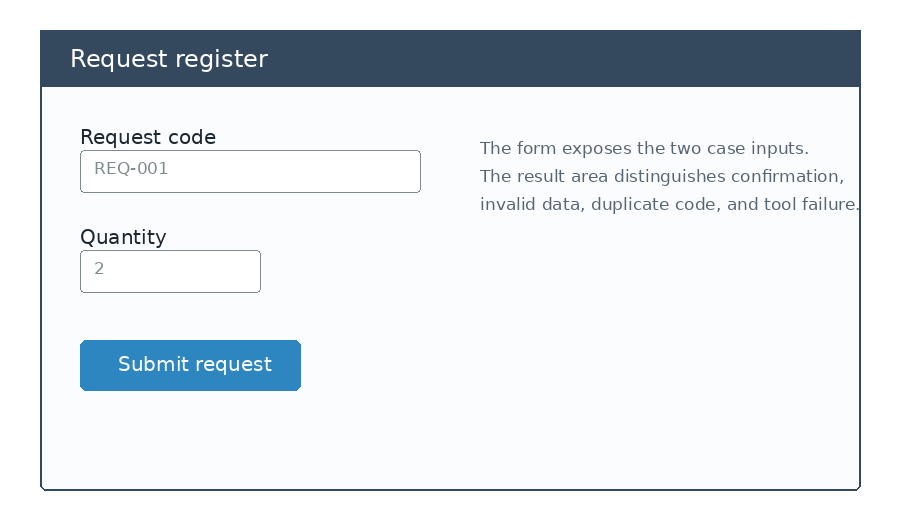
\includegraphics[width=0.62\linewidth]{assets/request-form.png}
\end{figure}
\begin{atlastext}{T000155}
Wireframe with Request code, Quantity, and Submit request.
\end{atlastext}
\AtlasMetaLine{Alternative text}{}
\begin{atlastext}{T000156}
A form with a Request code field, a Quantity field, and a Submit request button.
\end{atlastext}
\AtlasMetaLine{Assumptions}{ASM-\allowbreak{}REQUEST-\allowbreak{}STORE-\allowbreak{}UNIQUE}
\AtlasMetaLine{Sources}{SRC-\allowbreak{}REQUEST-\allowbreak{}BRIEF}
\AtlasMetaLine{Open issues}{OI-\allowbreak{}REQUEST-\allowbreak{}LATENCY}
\AtlasAppendixHeading{Appendix: graphs}
\begin{AtlasCatalog}
\hyperlink{technical-GRAPH-VLD-REQUEST-QUANTITY}{GRAPH-\allowbreak{}VLD-\allowbreak{}REQUEST-\allowbreak{}QUANTITY} & validation & \hyperlink{VLD-REQUEST-QUANTITY}{VLD-\allowbreak{}REQUEST-\allowbreak{}QUANTITY}; \hyperlink{figure-GRAPH-VLD-REQUEST-QUANTITY}{Figure}\\
\hyperlink{technical-GRAPH-REQUEST-SUBMIT}{GRAPH-\allowbreak{}REQUEST-\allowbreak{}SUBMIT} & use\_\allowbreak{}case & \hyperlink{UC-REQUEST-SUBMIT}{UC-\allowbreak{}REQUEST-\allowbreak{}SUBMIT}; \hyperlink{figure-GRAPH-REQUEST-SUBMIT}{Figure}\\
\hyperlink{technical-GRAPH-VLD-REQUEST-CODE}{GRAPH-\allowbreak{}VLD-\allowbreak{}REQUEST-\allowbreak{}CODE} & validation & \hyperlink{VLD-REQUEST-CODE}{VLD-\allowbreak{}REQUEST-\allowbreak{}CODE}; \hyperlink{figure-GRAPH-VLD-REQUEST-CODE}{Figure}\\
\end{AtlasCatalog}
\par\Needspace{8\baselineskip}\hypertarget{technical-GRAPH-VLD-REQUEST-QUANTITY}{}\AtlasSubheading{Graph \texttt{GRAPH-\allowbreak{}VLD-\allowbreak{}REQUEST-\allowbreak{}QUANTITY}}
\begin{atlastext}{T000157}
Quantity validation
\end{atlastext}
\AtlasMetaLine{Kind}{flow}
\par\Needspace{10\baselineskip}\AtlasLabel{Nodes}
\begin{AtlasCatalog}
\hypertarget{N-VLD-REQ-START}{}N-\allowbreak{}VLD-\allowbreak{}REQ-\allowbreak{}START & Type: start & Label: \AtlasCell{T000158}{Start}\newline{}Requirement refs: none\\\addlinespace[.35em]
\hypertarget{N-VLD-REQ-READ}{}N-\allowbreak{}VLD-\allowbreak{}REQ-\allowbreak{}READ & Type: action & Label: \AtlasCell{T000159}{Read quantity}\newline{}Requirement refs: none\\\addlinespace[.35em]
\hypertarget{N-VLD-REQ-TYPE}{}N-\allowbreak{}VLD-\allowbreak{}REQ-\allowbreak{}TYPE & Type: decision & Label: \AtlasCell{T000160}{Integer?}\newline{}Requirement refs: none\\\addlinespace[.35em]
\hypertarget{N-VLD-REQ-MIN}{}N-\allowbreak{}VLD-\allowbreak{}REQ-\allowbreak{}MIN & Type: decision & Label: \AtlasCell{T000161}{At least 1?}\newline{}Requirement refs: none\\\addlinespace[.35em]
\hypertarget{N-VLD-REQ-PASS}{}N-\allowbreak{}VLD-\allowbreak{}REQ-\allowbreak{}PASS & Type: result & Label: \AtlasCell{T000162}{Valid}\newline{}Requirement refs: none\\\addlinespace[.35em]
\hypertarget{N-VLD-REQ-FAIL-TYPE}{}N-\allowbreak{}VLD-\allowbreak{}REQ-\allowbreak{}FAIL-\allowbreak{}TYPE & Type: refusal & Label: \AtlasCell{T000163}{Invalid: not an integer}\newline{}Requirement refs: none\\\addlinespace[.35em]
\hypertarget{N-VLD-REQ-FAIL-MIN}{}N-\allowbreak{}VLD-\allowbreak{}REQ-\allowbreak{}FAIL-\allowbreak{}MIN & Type: refusal & Label: \AtlasCell{T000164}{Invalid: less than 1}\newline{}Requirement refs: none\\\addlinespace[.35em]
\end{AtlasCatalog}
\par\Needspace{10\baselineskip}\AtlasLabel{Edges}
\begin{AtlasCatalog}
\hypertarget{E-VLD-REQ-1}{}E-\allowbreak{}VLD-\allowbreak{}REQ-\allowbreak{}1 & From: N-\allowbreak{}VLD-\allowbreak{}REQ-\allowbreak{}START\newline{}To: N-\allowbreak{}VLD-\allowbreak{}REQ-\allowbreak{}READ & Requirement refs: none\\\addlinespace[.35em]
\hypertarget{E-VLD-REQ-2}{}E-\allowbreak{}VLD-\allowbreak{}REQ-\allowbreak{}2 & From: N-\allowbreak{}VLD-\allowbreak{}REQ-\allowbreak{}READ\newline{}To: N-\allowbreak{}VLD-\allowbreak{}REQ-\allowbreak{}TYPE & Requirement refs: none\\\addlinespace[.35em]
\hypertarget{E-VLD-REQ-3}{}E-\allowbreak{}VLD-\allowbreak{}REQ-\allowbreak{}3 & From: N-\allowbreak{}VLD-\allowbreak{}REQ-\allowbreak{}TYPE\newline{}To: N-\allowbreak{}VLD-\allowbreak{}REQ-\allowbreak{}FAIL-\allowbreak{}TYPE & Requirement refs: none\newline{}Label: \AtlasCell{T000165}{no}\\\addlinespace[.35em]
\hypertarget{E-VLD-REQ-4}{}E-\allowbreak{}VLD-\allowbreak{}REQ-\allowbreak{}4 & From: N-\allowbreak{}VLD-\allowbreak{}REQ-\allowbreak{}TYPE\newline{}To: N-\allowbreak{}VLD-\allowbreak{}REQ-\allowbreak{}MIN & Requirement refs: none\newline{}Label: \AtlasCell{T000166}{yes}\\\addlinespace[.35em]
\hypertarget{E-VLD-REQ-5}{}E-\allowbreak{}VLD-\allowbreak{}REQ-\allowbreak{}5 & From: N-\allowbreak{}VLD-\allowbreak{}REQ-\allowbreak{}MIN\newline{}To: N-\allowbreak{}VLD-\allowbreak{}REQ-\allowbreak{}FAIL-\allowbreak{}MIN & Requirement refs: none\newline{}Label: \AtlasCell{T000167}{no}\\\addlinespace[.35em]
\hypertarget{E-VLD-REQ-6}{}E-\allowbreak{}VLD-\allowbreak{}REQ-\allowbreak{}6 & From: N-\allowbreak{}VLD-\allowbreak{}REQ-\allowbreak{}MIN\newline{}To: N-\allowbreak{}VLD-\allowbreak{}REQ-\allowbreak{}PASS & Requirement refs: none\newline{}Label: \AtlasCell{T000168}{yes}\\\addlinespace[.35em]
\end{AtlasCatalog}
\begin{atlasderived}{DERIVED-GRAPH-GRAPH-VLD-REQUEST-QUANTITY}
Topology of GRAPH-VLD-REQUEST-QUANTITY:

Nodes:
- N-VLD-REQ-START (start)
- N-VLD-REQ-READ (action)
- N-VLD-REQ-TYPE (decision)
- N-VLD-REQ-MIN (decision)
- N-VLD-REQ-PASS (result)
- N-VLD-REQ-FAIL-TYPE (refusal)
- N-VLD-REQ-FAIL-MIN (refusal)

Edges:
- E-VLD-REQ-1: N-VLD-REQ-START -> N-VLD-REQ-READ
- E-VLD-REQ-2: N-VLD-REQ-READ -> N-VLD-REQ-TYPE
- E-VLD-REQ-3: N-VLD-REQ-TYPE -> N-VLD-REQ-FAIL-TYPE
- E-VLD-REQ-4: N-VLD-REQ-TYPE -> N-VLD-REQ-MIN
- E-VLD-REQ-5: N-VLD-REQ-MIN -> N-VLD-REQ-FAIL-MIN
- E-VLD-REQ-6: N-VLD-REQ-MIN -> N-VLD-REQ-PASS
\end{atlasderived}
\AtlasMetaLine{Figure}{\hyperlink{figure-GRAPH-VLD-REQUEST-QUANTITY}{GRAPH-\allowbreak{}VLD-\allowbreak{}REQUEST-\allowbreak{}QUANTITY}}
\par\Needspace{8\baselineskip}\hypertarget{technical-GRAPH-REQUEST-SUBMIT}{}\AtlasSubheading{Graph \texttt{GRAPH-\allowbreak{}REQUEST-\allowbreak{}SUBMIT}}
\begin{atlastext}{T000169}
Submit request
\end{atlastext}
\AtlasMetaLine{Kind}{flow}
\par\Needspace{10\baselineskip}\AtlasLabel{Nodes}
\begin{AtlasCatalog}
\hypertarget{N-REQ-START}{}N-\allowbreak{}REQ-\allowbreak{}START & Type: start & Label: \AtlasCell{T000170}{Start}\newline{}Requirement refs: none\\\addlinespace[.35em]
\hypertarget{N-REQ-PERM}{}N-\allowbreak{}REQ-\allowbreak{}PERM & Type: decision & Label: \AtlasCell{T000171}{Actor permitted?}\newline{}Requirement refs: RF-\allowbreak{}REQUEST-\allowbreak{}01\\\addlinespace[.35em]
\hypertarget{N-REQ-DENY}{}N-\allowbreak{}REQ-\allowbreak{}DENY & Type: refusal & Label: \AtlasCell{T000172}{Refuse: actor not permitted}\newline{}Requirement refs: RF-\allowbreak{}REQUEST-\allowbreak{}01\\\addlinespace[.35em]
\hypertarget{N-REQ-VALIDATE}{}N-\allowbreak{}REQ-\allowbreak{}VALIDATE & Type: validation & Label: \AtlasCell{T000173}{Apply VLD-REQUEST-QUANTITY}\newline{}Requirement refs: RF-\allowbreak{}REQUEST-\allowbreak{}02\newline{}Call: Kind: validation; Identifier: VLD-\allowbreak{}REQUEST-\allowbreak{}QUANTITY\\\addlinespace[.35em]
\hypertarget{N-REQ-QTYDEC}{}N-\allowbreak{}REQ-\allowbreak{}QTYDEC & Type: decision & Label: \AtlasCell{T000174}{Quantity valid?}\newline{}Requirement refs: RF-\allowbreak{}REQUEST-\allowbreak{}02\\\addlinespace[.35em]
\hypertarget{N-REQ-INVALID}{}N-\allowbreak{}REQ-\allowbreak{}INVALID & Type: refusal & Label: \AtlasCell{T000175}{Invalid code or quantity}\newline{}Requirement refs: RF-\allowbreak{}REQUEST-\allowbreak{}02; RF-\allowbreak{}REQUEST-\allowbreak{}07\\\addlinespace[.35em]
\hypertarget{N-REQ-STORE}{}N-\allowbreak{}REQ-\allowbreak{}STORE & Type: operation & Label: \AtlasCell{T000176}{Store request}\newline{}Requirement refs: RF-\allowbreak{}REQUEST-\allowbreak{}03\newline{}Call: Kind: operation; Identifier: OP-\allowbreak{}REQUEST-\allowbreak{}STORE\\\addlinespace[.35em]
\hypertarget{N-REQ-STOREERROR}{}N-\allowbreak{}REQ-\allowbreak{}STOREERROR & Type: failure & Label: \AtlasCell{T000177}{Report STORE\AtlasCharUnderscore{}UNAVAILABLE}\newline{}Requirement refs: RF-\allowbreak{}REQUEST-\allowbreak{}04\\\addlinespace[.35em]
\hypertarget{N-REQ-SUCCESS}{}N-\allowbreak{}REQ-\allowbreak{}SUCCESS & Type: result & Label: \AtlasCell{T000178}{Request confirmed}\newline{}Requirement refs: RF-\allowbreak{}REQUEST-\allowbreak{}05\\\addlinespace[.35em]
\hypertarget{N-REQ-DUPLICATE}{}N-\allowbreak{}REQ-\allowbreak{}DUPLICATE & Type: refusal & Label: \AtlasCell{T000179}{Duplicate code; no change}\newline{}Requirement refs: RF-\allowbreak{}REQUEST-\allowbreak{}06\\\addlinespace[.35em]
\hypertarget{N-REQ-CODE}{}N-\allowbreak{}REQ-\allowbreak{}CODE & Type: validation & Label: \AtlasCell{T000180}{Apply code validity}\newline{}Requirement refs: RF-\allowbreak{}REQUEST-\allowbreak{}07\newline{}Call: Kind: validation; Identifier: VLD-\allowbreak{}REQUEST-\allowbreak{}CODE\\\addlinespace[.35em]
\hypertarget{N-REQ-CODE-VALID}{}N-\allowbreak{}REQ-\allowbreak{}CODE-\allowbreak{}VALID & Type: decision & Label: \AtlasCell{T000181}{Code valid?}\newline{}Requirement refs: RF-\allowbreak{}REQUEST-\allowbreak{}07\\\addlinespace[.35em]
\end{AtlasCatalog}
\par\Needspace{10\baselineskip}\AtlasLabel{Edges}
\begin{AtlasCatalog}
\hypertarget{E-REQ-1}{}E-\allowbreak{}REQ-\allowbreak{}1 & From: N-\allowbreak{}REQ-\allowbreak{}START\newline{}To: N-\allowbreak{}REQ-\allowbreak{}PERM & Requirement refs: none\\\addlinespace[.35em]
\hypertarget{E-REQ-2}{}E-\allowbreak{}REQ-\allowbreak{}2 & From: N-\allowbreak{}REQ-\allowbreak{}PERM\newline{}To: N-\allowbreak{}REQ-\allowbreak{}DENY & Requirement refs: RF-\allowbreak{}REQUEST-\allowbreak{}01\newline{}Label: \AtlasCell{T000182}{no}\\\addlinespace[.35em]
\hypertarget{E-REQ-3}{}E-\allowbreak{}REQ-\allowbreak{}3 & From: N-\allowbreak{}REQ-\allowbreak{}PERM\newline{}To: N-\allowbreak{}REQ-\allowbreak{}CODE & Requirement refs: none\newline{}Label: \AtlasCell{T000183}{yes}\\\addlinespace[.35em]
\hypertarget{E-REQ-4}{}E-\allowbreak{}REQ-\allowbreak{}4 & From: N-\allowbreak{}REQ-\allowbreak{}VALIDATE\newline{}To: N-\allowbreak{}REQ-\allowbreak{}QTYDEC & Requirement refs: RF-\allowbreak{}REQUEST-\allowbreak{}02\\\addlinespace[.35em]
\hypertarget{E-REQ-5}{}E-\allowbreak{}REQ-\allowbreak{}5 & From: N-\allowbreak{}REQ-\allowbreak{}QTYDEC\newline{}To: N-\allowbreak{}REQ-\allowbreak{}INVALID & Requirement refs: RF-\allowbreak{}REQUEST-\allowbreak{}02\newline{}Label: \AtlasCell{T000184}{fail}\\\addlinespace[.35em]
\hypertarget{E-REQ-6}{}E-\allowbreak{}REQ-\allowbreak{}6 & From: N-\allowbreak{}REQ-\allowbreak{}QTYDEC\newline{}To: N-\allowbreak{}REQ-\allowbreak{}STORE & Requirement refs: RF-\allowbreak{}REQUEST-\allowbreak{}03\newline{}Label: \AtlasCell{T000185}{pass}\\\addlinespace[.35em]
\hypertarget{E-REQ-7}{}E-\allowbreak{}REQ-\allowbreak{}7 & From: N-\allowbreak{}REQ-\allowbreak{}STORE\newline{}To: N-\allowbreak{}REQ-\allowbreak{}SUCCESS & Requirement refs: RF-\allowbreak{}REQUEST-\allowbreak{}03; RF-\allowbreak{}REQUEST-\allowbreak{}05\newline{}Label: \AtlasCell{T000186}{stored}\\\addlinespace[.35em]
\hypertarget{E-REQ-8}{}E-\allowbreak{}REQ-\allowbreak{}8 & From: N-\allowbreak{}REQ-\allowbreak{}STORE\newline{}To: N-\allowbreak{}REQ-\allowbreak{}STOREERROR & Requirement refs: RF-\allowbreak{}REQUEST-\allowbreak{}04\newline{}Label: \AtlasCell{T000187}{STORE\AtlasCharUnderscore{}UNAVAILABLE}\\\addlinespace[.35em]
\hypertarget{E-REQ-DUPLICATE}{}E-\allowbreak{}REQ-\allowbreak{}DUPLICATE & From: N-\allowbreak{}REQ-\allowbreak{}STORE\newline{}To: N-\allowbreak{}REQ-\allowbreak{}DUPLICATE & Requirement refs: RF-\allowbreak{}REQUEST-\allowbreak{}06\newline{}Label: \AtlasCell{T000188}{DUPLICATE\AtlasCharUnderscore{}CODE}\\\addlinespace[.35em]
\hypertarget{E-REQ-CODE-1}{}E-\allowbreak{}REQ-\allowbreak{}CODE-\allowbreak{}1 & From: N-\allowbreak{}REQ-\allowbreak{}CODE\newline{}To: N-\allowbreak{}REQ-\allowbreak{}CODE-\allowbreak{}VALID & Requirement refs: none\\\addlinespace[.35em]
\hypertarget{E-REQ-CODE-2}{}E-\allowbreak{}REQ-\allowbreak{}CODE-\allowbreak{}2 & From: N-\allowbreak{}REQ-\allowbreak{}CODE-\allowbreak{}VALID\newline{}To: N-\allowbreak{}REQ-\allowbreak{}VALIDATE & Requirement refs: RF-\allowbreak{}REQUEST-\allowbreak{}07\newline{}Label: \AtlasCell{T000189}{pass}\\\addlinespace[.35em]
\hypertarget{E-REQ-CODE-3}{}E-\allowbreak{}REQ-\allowbreak{}CODE-\allowbreak{}3 & From: N-\allowbreak{}REQ-\allowbreak{}CODE-\allowbreak{}VALID\newline{}To: N-\allowbreak{}REQ-\allowbreak{}INVALID & Requirement refs: RF-\allowbreak{}REQUEST-\allowbreak{}07\newline{}Label: \AtlasCell{T000190}{fail}\\\addlinespace[.35em]
\end{AtlasCatalog}
\begin{atlasderived}{DERIVED-GRAPH-GRAPH-REQUEST-SUBMIT}
Topology of GRAPH-REQUEST-SUBMIT:

Nodes:
- N-REQ-START (start)
- N-REQ-PERM (decision)
- N-REQ-DENY (refusal)
- N-REQ-VALIDATE (validation)
- N-REQ-QTYDEC (decision)
- N-REQ-INVALID (refusal)
- N-REQ-STORE (operation)
- N-REQ-STOREERROR (failure)
- N-REQ-SUCCESS (result)
- N-REQ-DUPLICATE (refusal)
- N-REQ-CODE (validation)
- N-REQ-CODE-VALID (decision)

Edges:
- E-REQ-1: N-REQ-START -> N-REQ-PERM
- E-REQ-2: N-REQ-PERM -> N-REQ-DENY
- E-REQ-3: N-REQ-PERM -> N-REQ-CODE
- E-REQ-4: N-REQ-VALIDATE -> N-REQ-QTYDEC
- E-REQ-5: N-REQ-QTYDEC -> N-REQ-INVALID
- E-REQ-6: N-REQ-QTYDEC -> N-REQ-STORE
- E-REQ-7: N-REQ-STORE -> N-REQ-SUCCESS
- E-REQ-8: N-REQ-STORE -> N-REQ-STOREERROR
- E-REQ-DUPLICATE: N-REQ-STORE -> N-REQ-DUPLICATE
- E-REQ-CODE-1: N-REQ-CODE -> N-REQ-CODE-VALID
- E-REQ-CODE-2: N-REQ-CODE-VALID -> N-REQ-VALIDATE
- E-REQ-CODE-3: N-REQ-CODE-VALID -> N-REQ-INVALID
\end{atlasderived}
\AtlasMetaLine{Figure}{\hyperlink{figure-GRAPH-REQUEST-SUBMIT}{GRAPH-\allowbreak{}REQUEST-\allowbreak{}SUBMIT}}
\par\Needspace{8\baselineskip}\hypertarget{technical-GRAPH-VLD-REQUEST-CODE}{}\AtlasSubheading{Graph \texttt{GRAPH-\allowbreak{}VLD-\allowbreak{}REQUEST-\allowbreak{}CODE}}
\begin{atlastext}{T000191}
Request code validity
\end{atlastext}
\AtlasMetaLine{Kind}{flow}
\par\Needspace{10\baselineskip}\AtlasLabel{Nodes}
\begin{AtlasCatalog}
\hypertarget{N-VLD-REQ-CODE-START}{}N-\allowbreak{}VLD-\allowbreak{}REQ-\allowbreak{}CODE-\allowbreak{}START & Type: start & Label: \AtlasCell{T000192}{Receive code}\newline{}Requirement refs: none\\\addlinespace[.35em]
\hypertarget{N-VLD-REQ-CODE-CHECK}{}N-\allowbreak{}VLD-\allowbreak{}REQ-\allowbreak{}CODE-\allowbreak{}CHECK & Type: decision & Label: \AtlasCell{T000193}{Non-empty text?}\newline{}Requirement refs: none\\\addlinespace[.35em]
\hypertarget{N-VLD-REQ-CODE-PASS}{}N-\allowbreak{}VLD-\allowbreak{}REQ-\allowbreak{}CODE-\allowbreak{}PASS & Type: result & Label: \AtlasCell{T000194}{Pass unchanged}\newline{}Requirement refs: none\\\addlinespace[.35em]
\hypertarget{N-VLD-REQ-CODE-FAIL}{}N-\allowbreak{}VLD-\allowbreak{}REQ-\allowbreak{}CODE-\allowbreak{}FAIL & Type: refusal & Label: \AtlasCell{T000195}{Invalid code}\newline{}Requirement refs: none\\\addlinespace[.35em]
\end{AtlasCatalog}
\par\Needspace{10\baselineskip}\AtlasLabel{Edges}
\begin{AtlasCatalog}
\hypertarget{E-VLD-REQ-CODE-1}{}E-\allowbreak{}VLD-\allowbreak{}REQ-\allowbreak{}CODE-\allowbreak{}1 & From: N-\allowbreak{}VLD-\allowbreak{}REQ-\allowbreak{}CODE-\allowbreak{}START\newline{}To: N-\allowbreak{}VLD-\allowbreak{}REQ-\allowbreak{}CODE-\allowbreak{}CHECK & Requirement refs: none\\\addlinespace[.35em]
\hypertarget{E-VLD-REQ-CODE-2}{}E-\allowbreak{}VLD-\allowbreak{}REQ-\allowbreak{}CODE-\allowbreak{}2 & From: N-\allowbreak{}VLD-\allowbreak{}REQ-\allowbreak{}CODE-\allowbreak{}CHECK\newline{}To: N-\allowbreak{}VLD-\allowbreak{}REQ-\allowbreak{}CODE-\allowbreak{}PASS & Requirement refs: none\newline{}Label: \AtlasCell{T000196}{yes}\\\addlinespace[.35em]
\hypertarget{E-VLD-REQ-CODE-3}{}E-\allowbreak{}VLD-\allowbreak{}REQ-\allowbreak{}CODE-\allowbreak{}3 & From: N-\allowbreak{}VLD-\allowbreak{}REQ-\allowbreak{}CODE-\allowbreak{}CHECK\newline{}To: N-\allowbreak{}VLD-\allowbreak{}REQ-\allowbreak{}CODE-\allowbreak{}FAIL & Requirement refs: none\newline{}Label: \AtlasCell{T000197}{no}\\\addlinespace[.35em]
\end{AtlasCatalog}
\begin{atlasderived}{DERIVED-GRAPH-GRAPH-VLD-REQUEST-CODE}
Topology of GRAPH-VLD-REQUEST-CODE:

Nodes:
- N-VLD-REQ-CODE-START (start)
- N-VLD-REQ-CODE-CHECK (decision)
- N-VLD-REQ-CODE-PASS (result)
- N-VLD-REQ-CODE-FAIL (refusal)

Edges:
- E-VLD-REQ-CODE-1: N-VLD-REQ-CODE-START -> N-VLD-REQ-CODE-CHECK
- E-VLD-REQ-CODE-2: N-VLD-REQ-CODE-CHECK -> N-VLD-REQ-CODE-PASS
- E-VLD-REQ-CODE-3: N-VLD-REQ-CODE-CHECK -> N-VLD-REQ-CODE-FAIL
\end{atlasderived}
\AtlasMetaLine{Figure}{\hyperlink{figure-GRAPH-VLD-REQUEST-CODE}{GRAPH-\allowbreak{}VLD-\allowbreak{}REQUEST-\allowbreak{}CODE}}
\AtlasAppendixHeading{Appendix: resources}
\AtlasSubheading{Resource \texttt{RES-\allowbreak{}REQUEST-\allowbreak{}WIRE}}
\AtlasMetaLine{Path}{\texttt{assets/\allowbreak{}request-\allowbreak{}form.\allowbreak{}svg}}
\AtlasMetaLine{Media type}{image/\allowbreak{}svg+xml}
\AtlasMetaLine{SHA-256}{\texttt{f5a97fb7cb43af96\allowbreak{}81b2083fe1deebe3\allowbreak{}8bb3eda24adb947c\allowbreak{}3314317fc8a24de9\allowbreak{}}}
\AtlasLabel{Drawing source}
\begin{AtlasMetaTable}
\textcolor{AtlasMuted}{Path} & assets/\allowbreak{}request-\allowbreak{}form.\allowbreak{}svg & \textcolor{AtlasMuted}{Revision} & 1\\
\textcolor{AtlasMuted}{Tool} & scripts/\allowbreak{}build\_\allowbreak{}examples.\allowbreak{}py &  & \\
\end{AtlasMetaTable}
\AtlasLabel{Caption}
\begin{atlasparagraph}{T000198}
Request form wireframe: Request code, Quantity, and Submit request.
\end{atlasparagraph}
\AtlasLabel{Alternative text}
\begin{atlasparagraph}{T000199}
A form with a Request code field, a Quantity field, and a Submit request button. A result area reports confirmation, invalid data, duplicate code, or tool failure.
\end{atlasparagraph}
\AtlasLabel{Text present in the image}
\begin{atlasitem}{T000200}
Request code
\end{atlasitem}
\begin{atlasitem}{T000201}
Quantity
\end{atlasitem}
\begin{atlasitem}{T000202}
Submit request
\end{atlasitem}
\par\Needspace{10\baselineskip}\AtlasLabel{Variants}
\begin{AtlasCatalog}
 &  & Path: assets/\allowbreak{}request-\allowbreak{}form.\allowbreak{}png\newline{}Media type: image/\allowbreak{}png\newline{}Sha256: 5dd57bf8bccc9bcd\allowbreak{}9b68e1be1ea50163\allowbreak{}777caf93d83f6fbf\allowbreak{}ec1a099eb1d84347\allowbreak{}\newline{}Size: 22242\newline{}Relation: publication\newline{}Derived from: assets/\allowbreak{}request-\allowbreak{}form.\allowbreak{}svg\newline{}Producer: scripts/\allowbreak{}build\_\allowbreak{}examples.\allowbreak{}py\\\addlinespace[.35em]
\end{AtlasCatalog}
\AtlasSubheading{Resource \texttt{RES-\allowbreak{}REQUEST-\allowbreak{}FLOW}}
\AtlasMetaLine{Path}{\texttt{assets/\allowbreak{}request-\allowbreak{}flow.\allowbreak{}svg}}
\AtlasMetaLine{Media type}{image/\allowbreak{}svg+xml}
\AtlasMetaLine{SHA-256}{\texttt{71f3a97b667a8804\allowbreak{}1cc5812da8c8e7e1\allowbreak{}ddaced2f9c835e56\allowbreak{}c2c7d6d1b4252206\allowbreak{}}}
\AtlasLabel{Drawing source}
\begin{AtlasMetaTable}
\textcolor{AtlasMuted}{Path} & assets/\allowbreak{}request-\allowbreak{}flow.\allowbreak{}svg & \textcolor{AtlasMuted}{Revision} & 1286331986e92aa7\allowbreak{}0d90981f34da7aaa\allowbreak{}1dc45b09fa69106b\allowbreak{}4717745a2a095c0a\allowbreak{}\\
\textcolor{AtlasMuted}{Tool} & scripts/\allowbreak{}build\_\allowbreak{}examples.\allowbreak{}py &  & \\
\end{AtlasMetaTable}
\AtlasMetaLine{Derived from graph}{GRAPH-\allowbreak{}REQUEST-\allowbreak{}SUBMIT}
\AtlasLabel{Caption}
\begin{atlasparagraph}{T000203}
Submission flow with authorization, code and quantity validation, persistence, duplicate refusal and explicit write failure. The edge key identifies every structured edge.
\end{atlasparagraph}
\AtlasLabel{Alternative text}
\begin{atlasparagraph}{T000204}
Every node and edge of GRAPH-REQUEST-SUBMIT, with wrapped labels and an edge key. The text and graph records provide the complete accessible description.
\end{atlasparagraph}
\AtlasLabel{Text present in the image}
\begin{atlasitem}{T000205}
Start
\end{atlasitem}
\begin{atlasitem}{T000206}
Actor permitted?
\end{atlasitem}
\begin{atlasitem}{T000207}
Refuse: actor not permitted
\end{atlasitem}
\begin{atlasitem}{T000208}
Apply VLD-REQUEST-QUANTITY
\end{atlasitem}
\begin{atlasitem}{T000209}
Quantity valid?
\end{atlasitem}
\begin{atlasitem}{T000210}
Invalid code or quantity
\end{atlasitem}
\begin{atlasitem}{T000211}
Store request
\end{atlasitem}
\begin{atlasitem}{T000212}
Report STORE\AtlasCharUnderscore{}UNAVAILABLE
\end{atlasitem}
\begin{atlasitem}{T000213}
Request confirmed
\end{atlasitem}
\begin{atlasitem}{T000214}
Duplicate code; no change
\end{atlasitem}
\begin{atlasitem}{T000215}
Apply code validity
\end{atlasitem}
\begin{atlasitem}{T000216}
Code valid?
\end{atlasitem}
\begin{atlasitem}{T000217}
no
\end{atlasitem}
\begin{atlasitem}{T000218}
yes
\end{atlasitem}
\begin{atlasitem}{T000219}
fail
\end{atlasitem}
\begin{atlasitem}{T000220}
pass
\end{atlasitem}
\begin{atlasitem}{T000221}
stored
\end{atlasitem}
\begin{atlasitem}{T000222}
STORE\AtlasCharUnderscore{}UNAVAILABLE
\end{atlasitem}
\begin{atlasitem}{T000223}
DUPLICATE\AtlasCharUnderscore{}CODE
\end{atlasitem}
\begin{atlasitem}{T000224}
pass
\end{atlasitem}
\begin{atlasitem}{T000225}
fail
\end{atlasitem}
\par\Needspace{10\baselineskip}\AtlasLabel{Variants}
\begin{AtlasCatalog}
 &  & Path: assets/\allowbreak{}request-\allowbreak{}flow.\allowbreak{}png\newline{}Media type: image/\allowbreak{}png\newline{}Sha256: 53545111afdda2bc\allowbreak{}f5b113667ef14dc2\allowbreak{}233ca3f7e5e73074\allowbreak{}9d3f50473ed81f8b\allowbreak{}\newline{}Size: 73547\newline{}Relation: publication\newline{}Derived from: assets/\allowbreak{}request-\allowbreak{}flow.\allowbreak{}svg\newline{}Producer: scripts/\allowbreak{}build\_\allowbreak{}examples.\allowbreak{}py\\\addlinespace[.35em]
\end{AtlasCatalog}
\AtlasAppendixHeading{Appendix: assumptions}
\AtlasSubheading{\texttt{ASM-\allowbreak{}REQUEST-\allowbreak{}STORE-\allowbreak{}UNIQUE}}
\AtlasLabel{Statement}
\begin{atlasparagraph}{T000226}
A future implementation of the request store can enforce code uniqueness atomically.
\end{atlasparagraph}
\begin{AtlasMetaTable}
\textcolor{AtlasMuted}{Status} & open &  & \\
\end{AtlasMetaTable}
\AtlasMetaLine{Affected}{TOL-\allowbreak{}REQUEST-\allowbreak{}STORE, UC-\allowbreak{}REQUEST-\allowbreak{}SUBMIT}
\AtlasAppendixHeading{Appendix: decisions}
\AtlasSubheading{\texttt{DEC-\allowbreak{}MIN-\allowbreak{}TOOL-\allowbreak{}ABSTRACTION}}
\begin{AtlasMetaTable}
\textcolor{AtlasMuted}{Title} & \AtlasCell{T000227}{Keep the store abstract} &  & \\
\end{AtlasMetaTable}
\AtlasLabel{Context}
\begin{atlasparagraph}{T000228}
The example needs persistence but must not choose a technology.
\end{atlasparagraph}
\AtlasLabel{Decision}
\begin{atlasparagraph}{T000229}
Define OP-REQUEST-STORE as a tool contract only.
\end{atlasparagraph}
\AtlasLabel{Alternatives}
\begin{atlasparagraph}{T000230}
Specify SQLite tables and SQL statements.
\end{atlasparagraph}
\AtlasLabel{Consequences}
\begin{atlasparagraph}{T000231}
Implementations may choose storage, but must satisfy the contract.
\end{atlasparagraph}
\begin{AtlasMetaTable}
\textcolor{AtlasMuted}{Status} & accepted &  & \\
\end{AtlasMetaTable}
\AtlasMetaLine{Refs}{TOL-\allowbreak{}REQUEST-\allowbreak{}STORE}
\AtlasAppendixHeading{Appendix: open issues}
\AtlasSubheading{\texttt{OI-\allowbreak{}REQUEST-\allowbreak{}LATENCY}}
\begin{AtlasMetaTable}
\textcolor{AtlasMuted}{Title} & \AtlasCell{T000232}{Confirm the latency target} &  & \\
\end{AtlasMetaTable}
\AtlasLabel{Description}
\begin{atlasparagraph}{T000233}
The 2-second target is a verifiable example target; a production adoption must confirm it with stakeholders.
\end{atlasparagraph}
\begin{AtlasMetaTable}
\textcolor{AtlasMuted}{Status} & open &  & \\
\end{AtlasMetaTable}
\AtlasMetaLine{Refs}{RNF-\allowbreak{}REQUEST-\allowbreak{}01}
\AtlasAppendixHeading{Appendix: sources}
\AtlasSubheading{\texttt{SRC-\allowbreak{}REQUEST-\allowbreak{}BRIEF}}
\begin{AtlasMetaTable}
\textcolor{AtlasMuted}{Title} & \AtlasCell{T000234}{Illustrative request-register brief} & \textcolor{AtlasMuted}{Uri} & null\\
\textcolor{AtlasMuted}{Revision} & 2 & \textcolor{AtlasMuted}{Accessed} & null\\
\end{AtlasMetaTable}
\AtlasLabel{Note}
\begin{atlasparagraph}{T000235}
Internal teaching source; not a commissioned requirement.
\end{atlasparagraph}
\begin{atlasparagraph}{T000236}
The authorization policy, interaction sketches, and quality targets are didactic choices, not observed business facts.
\end{atlasparagraph}
\AtlasAppendixHeading{Appendix: history}
\AtlasSubheading{\texttt{HIST-\allowbreak{}REQUEST-\allowbreak{}01}}
\begin{AtlasMetaTable}
\textcolor{AtlasMuted}{Version} & 1 & \textcolor{AtlasMuted}{Date} & 2026-\allowbreak{}10-\allowbreak{}25\\
\end{AtlasMetaTable}
\AtlasLabel{Description}
\begin{atlasparagraph}{T000237}
Initial reference example for the first Atlas Specifications edition, Alpha-v0.1.0. This synthetic example demonstrates the model and its representations; it does not assert stakeholder approval or execution of the described business application.
\end{atlasparagraph}
\AtlasSubheading{\texttt{HIST-\allowbreak{}MIGRATION-\allowbreak{}STABLE}}
\begin{AtlasMetaTable}
\textcolor{AtlasMuted}{Version} & 2 & \textcolor{AtlasMuted}{Date} & 2026-\allowbreak{}10-\allowbreak{}25\\
\end{AtlasMetaTable}
\AtlasLabel{Description}
\begin{atlasparagraph}{T000238}
Explicit editorial migration from Atlas Alpha-v0.1.0 revision 1 to Atlas Stable-v1.0.0 revision 2. Model/profile/envelope and producer identities change; existing concept IDs, domain contracts, authored history and resources are retained. This is not format conversion, a Needs-to-L1 derivation, or new stakeholder approval.
\end{atlasparagraph}
\begin{atlasderived}{DERIVED-SUMMARY}
Derived summary: 5 sections; 1 actors; 1 entities; 1 tools; 1 use cases; 1 boundaries; 3 graphs; 2 resources.
\end{atlasderived}
%
% atlas:structure:begin
% {
%   "document_id": "ATLAS-EX-MINIMAL",
%   "title": {
%     "@text": "T000001"
%   },
%   "revision": "2",
%   "spec_version": "Stable-v1.0.0",
%   "profile_version": "Stable-v1.0.0",
%   "translator_version": "1.0.0",
%   "language": "en",
%   "status": "draft",
%   "authors": [
%     {
%       "name": {
%         "@text": "T000002"
%       },
%       "role": {
%         "@text": "T000003"
%       }
%     }
%   ],
%   "created": "2026-10-25",
%   "updated": "2026-10-25",
%   "subtitle": {
%     "@text": "T000004"
%   },
%   "keywords": [
%     {
%       "@text": "T000005"
%     },
%     {
%       "@text": "T000006"
%     },
%     {
%       "@text": "T000007"
%     },
%     {
%       "@text": "T000008"
%     }
%   ],
%   "structure": [
%     {
%       "id": "SEC-MIN-CONTEXT",
%       "level": 1,
%       "title": {
%         "@text": "T000009"
%       },
%       "blocks": [
%         {
%           "type": "paragraph",
%           "@text": "T000010"
%         },
%         {
%           "type": "paragraph",
%           "@text": "T000011"
%         },
%         {
%           "type": "note",
%           "@text": "T000012"
%         },
%         {
%           "type": "paragraph",
%           "@text": "T000013"
%         }
%       ],
%       "items": [
%         "ACT-REQUESTER",
%         "VOC-REQUEST-CODE"
%       ]
%     },
%     {
%       "id": "SEC-MIN-ENTITIES",
%       "level": 1,
%       "title": {
%         "@text": "T000014"
%       },
%       "blocks": [
%         {
%           "type": "paragraph",
%           "@text": "T000015"
%         }
%       ],
%       "items": [
%         "ENT-REQUEST"
%       ]
%     },
%     {
%       "id": "SEC-MIN-TOOLS",
%       "level": 1,
%       "title": {
%         "@text": "T000016"
%       },
%       "blocks": [
%         {
%           "type": "paragraph",
%           "@text": "T000017"
%         }
%       ],
%       "items": [
%         "TOL-REQUEST-STORE"
%       ]
%     },
%     {
%       "id": "SEC-MIN-CASES",
%       "level": 1,
%       "title": {
%         "@text": "T000018"
%       },
%       "blocks": [
%         {
%           "type": "paragraph",
%           "@text": "T000019"
%         }
%       ],
%       "items": [
%         "UC-REQUEST-SUBMIT"
%       ]
%     },
%     {
%       "id": "SEC-MIN-BOUNDARIES",
%       "level": 1,
%       "title": {
%         "@text": "T000020"
%       },
%       "blocks": [
%         {
%           "type": "paragraph",
%           "@text": "T000021"
%         }
%       ],
%       "items": [
%         "BND-REQUEST-WEB"
%       ]
%     }
%   ],
%   "actors": [
%     {
%       "id": "ACT-REQUESTER",
%       "name": {
%         "@text": "T000022"
%       },
%       "kind": "person",
%       "description": [
%         {
%           "type": "paragraph",
%           "@text": "T000023"
%         }
%       ]
%     }
%   ],
%   "vocabulary": [
%     {
%       "id": "VOC-REQUEST-CODE",
%       "term": {
%         "@text": "T000024"
%       },
%       "definition": [
%         {
%           "type": "paragraph",
%           "@text": "T000025"
%         }
%       ],
%       "synonyms": []
%     }
%   ],
%   "types": [],
%   "entities": [
%     {
%       "id": "ENT-REQUEST",
%       "name": {
%         "@text": "T000026"
%       },
%       "meaning": [
%         {
%           "type": "paragraph",
%           "@text": "T000027"
%         }
%       ],
%       "identity": {
%         "description": [
%           {
%             "type": "paragraph",
%             "@text": "T000028"
%           }
%         ],
%         "fields": [
%           "FLD-REQUEST-CODE"
%         ]
%       },
%       "fields": [
%         {
%           "id": "FLD-REQUEST-CODE",
%           "name": {
%             "@text": "T000029"
%           },
%           "type": "text",
%           "cardinality": "1",
%           "required": true,
%           "description": [
%             {
%               "type": "paragraph",
%               "@text": "T000030"
%             }
%           ],
%           "constraints": [
%             {
%               "type": "paragraph",
%               "@text": "T000031"
%             }
%           ],
%           "examples": {
%             "valid": [
%               {
%                 "@text": "T000032"
%               },
%               {
%                 "@text": "T000033"
%               }
%             ],
%             "invalid": [
%               {
%                 "@text": "T000034"
%               }
%             ]
%           }
%         },
%         {
%           "id": "FLD-REQUEST-QUANTITY",
%           "name": {
%             "@text": "T000035"
%           },
%           "type": "integer",
%           "cardinality": "1",
%           "required": true,
%           "description": [
%             {
%               "type": "paragraph",
%               "@text": "T000036"
%             }
%           ],
%           "constraints": [
%             {
%               "type": "paragraph",
%               "@text": "T000037"
%             }
%           ],
%           "examples": {
%             "valid": [
%               {
%                 "@text": "T000038"
%               },
%               {
%                 "@text": "T000039"
%               }
%             ],
%             "invalid": [
%               {
%                 "@text": "T000040"
%               },
%               {
%                 "@text": "T000041"
%               }
%             ]
%           }
%         }
%       ],
%       "relationships": [],
%       "states": [],
%       "transitions": [],
%       "validations": [
%         {
%           "id": "VLD-REQUEST-QUANTITY",
%           "name": {
%             "@text": "T000042"
%           },
%           "scope": "field",
%           "statement": [
%             {
%               "type": "paragraph",
%               "@text": "T000043"
%             }
%           ],
%           "inputs": [
%             {
%               "name": {
%                 "@text": "T000044"
%               },
%               "source": "field",
%               "meaning": [
%                 {
%                   "type": "paragraph",
%                   "@text": "T000045"
%                 }
%               ]
%             }
%           ],
%           "conditions": [
%             {
%               "id": "C-VLD-REQ-INT",
%               "condition": {
%                 "@text": "T000046"
%               },
%               "meaning": [
%                 {
%                   "type": "paragraph",
%                   "@text": "T000047"
%                 }
%               ]
%             },
%             {
%               "id": "C-VLD-REQ-MIN",
%               "condition": {
%                 "@text": "T000048"
%               },
%               "meaning": [
%                 {
%                   "type": "paragraph",
%                   "@text": "T000049"
%                 }
%               ]
%             }
%           ],
%           "results": [
%             {
%               "outcome": "pass",
%               "description": [
%                 {
%                   "type": "paragraph",
%                   "@text": "T000050"
%                 }
%               ]
%             },
%             {
%               "outcome": "fail",
%               "description": [
%                 {
%                   "type": "paragraph",
%                   "@text": "T000051"
%                 }
%               ]
%             }
%           ],
%           "flow": "GRAPH-VLD-REQUEST-QUANTITY"
%         },
%         {
%           "id": "VLD-REQUEST-CODE",
%           "name": {
%             "@text": "T000052"
%           },
%           "scope": "field",
%           "statement": [
%             {
%               "type": "paragraph",
%               "@text": "T000053"
%             }
%           ],
%           "inputs": [
%             {
%               "name": {
%                 "@text": "T000054"
%               },
%               "source": "field",
%               "meaning": [
%                 {
%                   "type": "paragraph",
%                   "@text": "T000055"
%                 }
%               ]
%             }
%           ],
%           "conditions": [
%             {
%               "id": "C-VLD-REQ-CODE-NONEMPTY",
%               "condition": {
%                 "@text": "T000056"
%               },
%               "meaning": [
%                 {
%                   "type": "paragraph",
%                   "@text": "T000057"
%                 }
%               ]
%             }
%           ],
%           "results": [
%             {
%               "outcome": "pass",
%               "description": [
%                 {
%                   "type": "paragraph",
%                   "@text": "T000058"
%                 }
%               ]
%             },
%             {
%               "outcome": "fail",
%               "description": [
%                 {
%                   "type": "paragraph",
%                   "@text": "T000059"
%                 }
%               ]
%             }
%           ],
%           "flow": "GRAPH-VLD-REQUEST-CODE"
%         }
%       ],
%       "examples": [
%         {
%           "id": "EX-REQUEST-VALID",
%           "kind": "valid",
%           "description": [
%             {
%               "type": "paragraph",
%               "@text": "T000060"
%             }
%           ],
%           "data": {
%             "code": "REQ-001",
%             "quantity": 2
%           }
%         },
%         {
%           "id": "EX-REQUEST-INVALID",
%           "kind": "invalid",
%           "description": [
%             {
%               "type": "paragraph",
%               "@text": "T000061"
%             }
%           ],
%           "data": {
%             "code": "REQ-001",
%             "quantity": 0
%           }
%         }
%       ],
%       "assumptions": [
%         "ASM-REQUEST-STORE-UNIQUE"
%       ],
%       "open_issues": [
%         "OI-REQUEST-LATENCY"
%       ]
%     }
%   ],
%   "tools": [
%     {
%       "id": "TOL-REQUEST-STORE",
%       "name": {
%         "@text": "T000062"
%       },
%       "purpose": [
%         {
%           "type": "paragraph",
%           "@text": "T000063"
%         }
%       ],
%       "operations": [
%         {
%           "id": "OP-REQUEST-STORE",
%           "name": {
%             "@text": "T000064"
%           },
%           "purpose": [
%             {
%               "type": "paragraph",
%               "@text": "T000065"
%             }
%           ],
%           "inputs": [
%             {
%               "name": {
%                 "@text": "T000066"
%               },
%               "type": "text",
%               "meaning": [
%                 {
%                   "type": "paragraph",
%                   "@text": "T000067"
%                 }
%               ],
%               "required": true
%             },
%             {
%               "name": {
%                 "@text": "T000068"
%               },
%               "type": "integer",
%               "meaning": [
%                 {
%                   "type": "paragraph",
%                   "@text": "T000069"
%                 }
%               ],
%               "required": true
%             }
%           ],
%           "conditions": [
%             {
%               "type": "paragraph",
%               "@text": "T000070"
%             },
%             {
%               "type": "paragraph",
%               "@text": "T000071"
%             },
%             {
%               "type": "paragraph",
%               "@text": "T000072"
%             }
%           ],
%           "results": [
%             {
%               "name": {
%                 "@text": "T000073"
%               },
%               "type": "REQUEST",
%               "meaning": [
%                 {
%                   "type": "paragraph",
%                   "@text": "T000074"
%                 }
%               ],
%               "guarantees": [
%                 {
%                   "type": "paragraph",
%                   "@text": "T000075"
%                 }
%               ]
%             }
%           ],
%           "effects": [
%             {
%               "type": "paragraph",
%               "@text": "T000076"
%             }
%           ],
%           "failures": [
%             {
%               "code": "DUPLICATE_CODE",
%               "meaning": [
%                 {
%                   "type": "paragraph",
%                   "@text": "T000077"
%                 }
%               ],
%               "consumer_distinction": [
%                 {
%                   "type": "paragraph",
%                   "@text": "T000078"
%                 }
%               ]
%             },
%             {
%               "code": "STORE_UNAVAILABLE",
%               "meaning": [
%                 {
%                   "type": "paragraph",
%                   "@text": "T000079"
%                 }
%               ],
%               "consumer_distinction": [
%                 {
%                   "type": "paragraph",
%                   "@text": "T000080"
%                 }
%               ]
%             }
%           ],
%           "guarantees": [
%             {
%               "type": "paragraph",
%               "@text": "T000081"
%             },
%             {
%               "type": "paragraph",
%               "@text": "T000082"
%             }
%           ]
%         }
%       ]
%     }
%   ],
%   "use_cases": [
%     {
%       "id": "UC-REQUEST-SUBMIT",
%       "name": {
%         "@text": "T000083"
%       },
%       "objective": [
%         {
%           "type": "paragraph",
%           "@text": "T000084"
%         }
%       ],
%       "actors": [
%         {
%           "actor": "ACT-REQUESTER",
%           "permission": {
%             "@text": "T000085"
%           },
%           "description": [
%             {
%               "type": "paragraph",
%               "@text": "T000086"
%             },
%             {
%               "type": "paragraph",
%               "@text": "T000087"
%             }
%           ]
%         }
%       ],
%       "trigger": [
%         {
%           "type": "paragraph",
%           "@text": "T000088"
%         }
%       ],
%       "context": [
%         {
%           "type": "paragraph",
%           "@text": "T000089"
%         },
%         {
%           "type": "paragraph",
%           "@text": "T000090"
%         },
%         {
%           "type": "paragraph",
%           "@text": "T000091"
%         }
%       ],
%       "inputs": [
%         {
%           "name": {
%             "@text": "T000092"
%           },
%           "type": "text",
%           "meaning": [
%             {
%               "type": "paragraph",
%               "@text": "T000093"
%             }
%           ],
%           "required": true
%         },
%         {
%           "name": {
%             "@text": "T000094"
%           },
%           "type": "integer",
%           "meaning": [
%             {
%               "type": "paragraph",
%               "@text": "T000095"
%             }
%           ],
%           "required": true
%         }
%       ],
%       "entry_conditions": [
%         {
%           "type": "paragraph",
%           "@text": "T000096"
%         }
%       ],
%       "entities": [
%         {
%           "entity": "ENT-REQUEST",
%           "validations": [
%             "VLD-REQUEST-QUANTITY",
%             "VLD-REQUEST-CODE"
%           ],
%           "purpose": [
%             {
%               "type": "paragraph",
%               "@text": "T000097"
%             }
%           ]
%         }
%       ],
%       "tools": [
%         {
%           "tool": "TOL-REQUEST-STORE",
%           "operation": "OP-REQUEST-STORE",
%           "purpose": [
%             {
%               "type": "paragraph",
%               "@text": "T000098"
%             }
%           ]
%         }
%       ],
%       "calls": [],
%       "outcomes": [
%         {
%           "id": "OUT-REQUEST-CONFIRMED",
%           "kind": "success",
%           "description": [
%             {
%               "type": "paragraph",
%               "@text": "T000099"
%             }
%           ],
%           "effects": [
%             {
%               "type": "paragraph",
%               "@text": "T000100"
%             }
%           ]
%         },
%         {
%           "id": "OUT-REQUEST-INVALID",
%           "kind": "refusal",
%           "description": [
%             {
%               "type": "paragraph",
%               "@text": "T000101"
%             }
%           ],
%           "effects": [
%             {
%               "type": "paragraph",
%               "@text": "T000102"
%             }
%           ]
%         },
%         {
%           "id": "OUT-REQUEST-DENIED",
%           "kind": "refusal",
%           "description": [
%             {
%               "type": "paragraph",
%               "@text": "T000103"
%             }
%           ],
%           "effects": [
%             {
%               "type": "paragraph",
%               "@text": "T000104"
%             }
%           ]
%         },
%         {
%           "id": "OUT-REQUEST-STORE-FAILURE",
%           "kind": "failure",
%           "description": [
%             {
%               "type": "paragraph",
%               "@text": "T000105"
%             }
%           ],
%           "effects": [
%             {
%               "type": "paragraph",
%               "@text": "T000106"
%             }
%           ]
%         },
%         {
%           "id": "OUT-REQUEST-DUPLICATE",
%           "kind": "refusal",
%           "description": [
%             {
%               "type": "paragraph",
%               "@text": "T000107"
%             }
%           ],
%           "effects": [
%             {
%               "type": "paragraph",
%               "@text": "T000108"
%             }
%           ]
%         }
%       ],
%       "functional_requirements": [
%         {
%           "id": "RF-REQUEST-01",
%           "statement": [
%             {
%               "type": "paragraph",
%               "@text": "T000109"
%             }
%           ],
%           "scope": "case",
%           "applies_to": [
%             "UC-REQUEST-SUBMIT",
%             "INT-REQUEST-SUBMIT"
%           ],
%           "flow_refs": [
%             "N-REQ-PERM",
%             "N-REQ-DENY",
%             "E-REQ-2"
%           ]
%         },
%         {
%           "id": "RF-REQUEST-02",
%           "statement": [
%             {
%               "type": "paragraph",
%               "@text": "T000110"
%             }
%           ],
%           "scope": "case",
%           "applies_to": [
%             "UC-REQUEST-SUBMIT",
%             "INT-REQUEST-SUBMIT"
%           ],
%           "flow_refs": [
%             "N-REQ-VALIDATE",
%             "N-REQ-QTYDEC",
%             "N-REQ-INVALID",
%             "E-REQ-4",
%             "E-REQ-5"
%           ]
%         },
%         {
%           "id": "RF-REQUEST-03",
%           "statement": [
%             {
%               "type": "paragraph",
%               "@text": "T000111"
%             }
%           ],
%           "scope": "operation",
%           "applies_to": [
%             "UC-REQUEST-SUBMIT",
%             "OP-REQUEST-STORE"
%           ],
%           "flow_refs": [
%             "N-REQ-STORE",
%             "E-REQ-6",
%             "E-REQ-7"
%           ]
%         },
%         {
%           "id": "RF-REQUEST-04",
%           "statement": [
%             {
%               "type": "paragraph",
%               "@text": "T000112"
%             },
%             {
%               "type": "paragraph",
%               "@text": "T000113"
%             }
%           ],
%           "scope": "operation",
%           "applies_to": [
%             "UC-REQUEST-SUBMIT",
%             "OP-REQUEST-STORE"
%           ],
%           "flow_refs": [
%             "N-REQ-STOREERROR",
%             "E-REQ-8"
%           ]
%         },
%         {
%           "id": "RF-REQUEST-05",
%           "statement": [
%             {
%               "type": "paragraph",
%               "@text": "T000114"
%             }
%           ],
%           "scope": "interaction",
%           "applies_to": [
%             "UC-REQUEST-SUBMIT",
%             "INT-REQUEST-SUBMIT"
%           ],
%           "flow_refs": [
%             "N-REQ-SUCCESS",
%             "E-REQ-7"
%           ]
%         },
%         {
%           "id": "RF-REQUEST-06",
%           "statement": [
%             {
%               "type": "paragraph",
%               "@text": "T000115"
%             }
%           ],
%           "scope": "operation",
%           "applies_to": [
%             "UC-REQUEST-SUBMIT",
%             "OP-REQUEST-STORE"
%           ],
%           "flow_refs": [
%             "N-REQ-DUPLICATE",
%             "E-REQ-DUPLICATE"
%           ]
%         },
%         {
%           "id": "RF-REQUEST-07",
%           "statement": [
%             {
%               "type": "paragraph",
%               "@text": "T000116"
%             }
%           ],
%           "scope": "case",
%           "applies_to": [
%             "UC-REQUEST-SUBMIT"
%           ],
%           "flow_refs": [
%             "N-REQ-INVALID",
%             "N-REQ-CODE",
%             "N-REQ-CODE-VALID",
%             "E-REQ-CODE-2",
%             "E-REQ-CODE-3"
%           ]
%         }
%       ],
%       "nonfunctional_requirements": [
%         {
%           "id": "RNF-REQUEST-01",
%           "scope": "interaction",
%           "applies_to": [
%             "INT-REQUEST-SUBMIT"
%           ],
%           "statement": [
%             {
%               "type": "paragraph",
%               "@text": "T000117"
%             }
%           ],
%           "criterion": [
%             {
%               "type": "paragraph",
%               "@text": "T000118"
%             }
%           ],
%           "verification": [
%             {
%               "type": "paragraph",
%               "@text": "T000119"
%             }
%           ],
%           "metric": {
%             "name": {
%               "@text": "T000120"
%             },
%             "unit": {
%               "@text": "T000121"
%             },
%             "target": "2",
%             "operator": "<="
%           },
%           "measurement": {
%             "start": [
%               {
%                 "type": "paragraph",
%                 "@text": "T000122"
%               }
%             ],
%             "end": [
%               {
%                 "type": "paragraph",
%                 "@text": "T000123"
%               }
%             ]
%           },
%           "references": [
%             "SRC-REQUEST-BRIEF"
%           ],
%           "applicability": [
%             {
%               "type": "paragraph",
%               "@text": "T000124"
%             }
%           ]
%         }
%       ],
%       "flows": {
%         "main": "GRAPH-REQUEST-SUBMIT",
%         "subflows": []
%       },
%       "flow_text": [
%         {
%           "type": "paragraph",
%           "@text": "T000125"
%         },
%         {
%           "type": "paragraph",
%           "@text": "T000126"
%         },
%         {
%           "type": "paragraph",
%           "@text": "T000127"
%         },
%         {
%           "type": "paragraph",
%           "@text": "T000128"
%         },
%         {
%           "type": "paragraph",
%           "@text": "T000129"
%         }
%       ],
%       "acceptance_criteria": [
%         {
%           "id": "AC-REQUEST-01",
%           "statement": [
%             {
%               "type": "paragraph",
%               "@text": "T000130"
%             }
%           ],
%           "verifies": [
%             "RF-REQUEST-02",
%             "RF-REQUEST-03",
%             "RF-REQUEST-05"
%           ]
%         },
%         {
%           "id": "AC-REQUEST-02",
%           "statement": [
%             {
%               "type": "paragraph",
%               "@text": "T000131"
%             }
%           ],
%           "verifies": [
%             "RF-REQUEST-02"
%           ]
%         },
%         {
%           "id": "AC-REQUEST-03",
%           "statement": [
%             {
%               "type": "paragraph",
%               "@text": "T000132"
%             }
%           ],
%           "verifies": [
%             "RF-REQUEST-01"
%           ]
%         },
%         {
%           "id": "AC-REQUEST-04",
%           "statement": [
%             {
%               "type": "paragraph",
%               "@text": "T000133"
%             }
%           ],
%           "verifies": [
%             "RF-REQUEST-06"
%           ]
%         },
%         {
%           "id": "AC-REQUEST-05",
%           "statement": [
%             {
%               "type": "paragraph",
%               "@text": "T000134"
%             }
%           ],
%           "verifies": [
%             "RF-REQUEST-04"
%           ]
%         },
%         {
%           "id": "AC-REQUEST-06",
%           "statement": [
%             {
%               "type": "paragraph",
%               "@text": "T000135"
%             }
%           ],
%           "verifies": [
%             "RF-REQUEST-07"
%           ]
%         },
%         {
%           "id": "AC-REQUEST-SUBMIT-QUALITY",
%           "statement": [
%             {
%               "type": "paragraph",
%               "@text": "T000136"
%             }
%           ],
%           "verifies": [
%             "RNF-REQUEST-01"
%           ]
%         }
%       ],
%       "traceability": [
%         {
%           "id": "TRC-REQUEST-01",
%           "source": "RF-REQUEST-02",
%           "targets": [
%             "VLD-REQUEST-QUANTITY",
%             "AC-REQUEST-02"
%           ],
%           "note": [
%             {
%               "type": "paragraph",
%               "@text": "T000137"
%             }
%           ]
%         },
%         {
%           "id": "TRC-REQUEST-02",
%           "source": "RF-REQUEST-03",
%           "targets": [
%             "OP-REQUEST-STORE",
%             "AC-REQUEST-01"
%           ],
%           "note": [
%             {
%               "type": "paragraph",
%               "@text": "T000138"
%             }
%           ]
%         },
%         {
%           "id": "TRC-REQUEST-SUBMIT-ORIGIN",
%           "source": "SRC-REQUEST-BRIEF",
%           "targets": [
%             "RF-REQUEST-01",
%             "RF-REQUEST-02",
%             "RF-REQUEST-03",
%             "RF-REQUEST-04",
%             "RF-REQUEST-05",
%             "RF-REQUEST-06",
%             "RF-REQUEST-07",
%             "RNF-REQUEST-01"
%           ],
%           "note": [
%             {
%               "type": "paragraph",
%               "@text": "T000139"
%             }
%           ]
%         }
%       ],
%       "assumptions": [
%         "ASM-REQUEST-STORE-UNIQUE"
%       ],
%       "sources": [
%         "SRC-REQUEST-BRIEF"
%       ],
%       "open_issues": [
%         "OI-REQUEST-LATENCY"
%       ]
%     }
%   ],
%   "boundaries": [
%     {
%       "id": "BND-REQUEST-WEB",
%       "name": {
%         "@text": "T000140"
%       },
%       "modality": "web",
%       "purpose": [
%         {
%           "type": "paragraph",
%           "@text": "T000141"
%         },
%         {
%           "type": "paragraph",
%           "@text": "T000142"
%         }
%       ],
%       "audience": [
%         {
%           "type": "paragraph",
%           "@text": "T000143"
%         }
%       ],
%       "interactions": [
%         {
%           "id": "INT-REQUEST-SUBMIT",
%           "name": {
%             "@text": "T000144"
%           },
%           "description": [
%             {
%               "type": "paragraph",
%               "@text": "T000145"
%             },
%             {
%               "type": "paragraph",
%               "@text": "T000146"
%             }
%           ],
%           "use_case": "UC-REQUEST-SUBMIT",
%           "trigger": [
%             {
%               "type": "paragraph",
%               "@text": "T000147"
%             }
%           ],
%           "input_mapping": [
%             {
%               "source": "form.code",
%               "target": "UC-REQUEST-SUBMIT.input.code",
%               "meaning": [
%                 {
%                   "type": "paragraph",
%                   "@text": "T000148"
%                 }
%               ]
%             },
%             {
%               "source": "form.quantity",
%               "target": "UC-REQUEST-SUBMIT.input.quantity",
%               "meaning": [
%                 {
%                   "type": "paragraph",
%                   "@text": "T000149"
%                 }
%               ]
%             }
%           ],
%           "result_mapping": [
%             {
%               "source": "OUT-REQUEST-CONFIRMED",
%               "target": "result.confirmation",
%               "meaning": [
%                 {
%                   "type": "paragraph",
%                   "@text": "T000150"
%                 }
%               ]
%             },
%             {
%               "source": "OUT-REQUEST-INVALID",
%               "target": "result.invalid_data",
%               "meaning": [
%                 {
%                   "type": "paragraph",
%                   "@text": "T000151"
%                 }
%               ]
%             },
%             {
%               "source": "OUT-REQUEST-STORE-FAILURE",
%               "target": "result.store_unavailable",
%               "meaning": [
%                 {
%                   "type": "paragraph",
%                   "@text": "T000152"
%                 }
%               ]
%             },
%             {
%               "source": "OUT-REQUEST-DENIED",
%               "target": "result.out-request-denied",
%               "meaning": [
%                 {
%                   "type": "paragraph",
%                   "@text": "T000153"
%                 }
%               ]
%             },
%             {
%               "source": "OUT-REQUEST-DUPLICATE",
%               "target": "result.out-request-duplicate",
%               "meaning": [
%                 {
%                   "type": "paragraph",
%                   "@text": "T000154"
%                 }
%               ]
%             }
%           ],
%           "requirement_refs": [
%             "RF-REQUEST-01",
%             "RF-REQUEST-02",
%             "RF-REQUEST-03",
%             "RF-REQUEST-04",
%             "RF-REQUEST-05",
%             "RF-REQUEST-06",
%             "RF-REQUEST-07"
%           ],
%           "resources": [
%             "RES-REQUEST-WIRE",
%             "RES-REQUEST-FLOW"
%           ],
%           "examples": [
%             {
%               "type": "figure",
%               "resource": "RES-REQUEST-WIRE",
%               "caption": {
%                 "@text": "T000155"
%               },
%               "alt": {
%                 "@text": "T000156"
%               }
%             }
%           ]
%         }
%       ],
%       "assumptions": [
%         "ASM-REQUEST-STORE-UNIQUE"
%       ],
%       "sources": [
%         "SRC-REQUEST-BRIEF"
%       ],
%       "open_issues": [
%         "OI-REQUEST-LATENCY"
%       ]
%     }
%   ],
%   "graphs": [
%     {
%       "id": "GRAPH-VLD-REQUEST-QUANTITY",
%       "kind": "flow",
%       "owner": {
%         "kind": "validation",
%         "id": "VLD-REQUEST-QUANTITY"
%       },
%       "title": {
%         "@text": "T000157"
%       },
%       "nodes": [
%         {
%           "id": "N-VLD-REQ-START",
%           "type": "start",
%           "label": {
%             "@text": "T000158"
%           },
%           "requirement_refs": []
%         },
%         {
%           "id": "N-VLD-REQ-READ",
%           "type": "action",
%           "label": {
%             "@text": "T000159"
%           },
%           "requirement_refs": []
%         },
%         {
%           "id": "N-VLD-REQ-TYPE",
%           "type": "decision",
%           "label": {
%             "@text": "T000160"
%           },
%           "requirement_refs": []
%         },
%         {
%           "id": "N-VLD-REQ-MIN",
%           "type": "decision",
%           "label": {
%             "@text": "T000161"
%           },
%           "requirement_refs": []
%         },
%         {
%           "id": "N-VLD-REQ-PASS",
%           "type": "result",
%           "label": {
%             "@text": "T000162"
%           },
%           "requirement_refs": []
%         },
%         {
%           "id": "N-VLD-REQ-FAIL-TYPE",
%           "type": "refusal",
%           "label": {
%             "@text": "T000163"
%           },
%           "requirement_refs": []
%         },
%         {
%           "id": "N-VLD-REQ-FAIL-MIN",
%           "type": "refusal",
%           "label": {
%             "@text": "T000164"
%           },
%           "requirement_refs": []
%         }
%       ],
%       "edges": [
%         {
%           "id": "E-VLD-REQ-1",
%           "from": "N-VLD-REQ-START",
%           "to": "N-VLD-REQ-READ",
%           "requirement_refs": []
%         },
%         {
%           "id": "E-VLD-REQ-2",
%           "from": "N-VLD-REQ-READ",
%           "to": "N-VLD-REQ-TYPE",
%           "requirement_refs": []
%         },
%         {
%           "id": "E-VLD-REQ-3",
%           "from": "N-VLD-REQ-TYPE",
%           "to": "N-VLD-REQ-FAIL-TYPE",
%           "requirement_refs": [],
%           "label": {
%             "@text": "T000165"
%           }
%         },
%         {
%           "id": "E-VLD-REQ-4",
%           "from": "N-VLD-REQ-TYPE",
%           "to": "N-VLD-REQ-MIN",
%           "requirement_refs": [],
%           "label": {
%             "@text": "T000166"
%           }
%         },
%         {
%           "id": "E-VLD-REQ-5",
%           "from": "N-VLD-REQ-MIN",
%           "to": "N-VLD-REQ-FAIL-MIN",
%           "requirement_refs": [],
%           "label": {
%             "@text": "T000167"
%           }
%         },
%         {
%           "id": "E-VLD-REQ-6",
%           "from": "N-VLD-REQ-MIN",
%           "to": "N-VLD-REQ-PASS",
%           "requirement_refs": [],
%           "label": {
%             "@text": "T000168"
%           }
%         }
%       ]
%     },
%     {
%       "id": "GRAPH-REQUEST-SUBMIT",
%       "kind": "flow",
%       "owner": {
%         "kind": "use_case",
%         "id": "UC-REQUEST-SUBMIT"
%       },
%       "title": {
%         "@text": "T000169"
%       },
%       "nodes": [
%         {
%           "id": "N-REQ-START",
%           "type": "start",
%           "label": {
%             "@text": "T000170"
%           },
%           "requirement_refs": []
%         },
%         {
%           "id": "N-REQ-PERM",
%           "type": "decision",
%           "label": {
%             "@text": "T000171"
%           },
%           "requirement_refs": [
%             "RF-REQUEST-01"
%           ]
%         },
%         {
%           "id": "N-REQ-DENY",
%           "type": "refusal",
%           "label": {
%             "@text": "T000172"
%           },
%           "requirement_refs": [
%             "RF-REQUEST-01"
%           ]
%         },
%         {
%           "id": "N-REQ-VALIDATE",
%           "type": "validation",
%           "label": {
%             "@text": "T000173"
%           },
%           "requirement_refs": [
%             "RF-REQUEST-02"
%           ],
%           "call": {
%             "kind": "validation",
%             "id": "VLD-REQUEST-QUANTITY"
%           }
%         },
%         {
%           "id": "N-REQ-QTYDEC",
%           "type": "decision",
%           "label": {
%             "@text": "T000174"
%           },
%           "requirement_refs": [
%             "RF-REQUEST-02"
%           ]
%         },
%         {
%           "id": "N-REQ-INVALID",
%           "type": "refusal",
%           "label": {
%             "@text": "T000175"
%           },
%           "requirement_refs": [
%             "RF-REQUEST-02",
%             "RF-REQUEST-07"
%           ]
%         },
%         {
%           "id": "N-REQ-STORE",
%           "type": "operation",
%           "label": {
%             "@text": "T000176"
%           },
%           "requirement_refs": [
%             "RF-REQUEST-03"
%           ],
%           "call": {
%             "kind": "operation",
%             "id": "OP-REQUEST-STORE"
%           }
%         },
%         {
%           "id": "N-REQ-STOREERROR",
%           "type": "failure",
%           "label": {
%             "@text": "T000177"
%           },
%           "requirement_refs": [
%             "RF-REQUEST-04"
%           ]
%         },
%         {
%           "id": "N-REQ-SUCCESS",
%           "type": "result",
%           "label": {
%             "@text": "T000178"
%           },
%           "requirement_refs": [
%             "RF-REQUEST-05"
%           ]
%         },
%         {
%           "id": "N-REQ-DUPLICATE",
%           "type": "refusal",
%           "label": {
%             "@text": "T000179"
%           },
%           "requirement_refs": [
%             "RF-REQUEST-06"
%           ]
%         },
%         {
%           "id": "N-REQ-CODE",
%           "type": "validation",
%           "label": {
%             "@text": "T000180"
%           },
%           "requirement_refs": [
%             "RF-REQUEST-07"
%           ],
%           "call": {
%             "kind": "validation",
%             "id": "VLD-REQUEST-CODE"
%           }
%         },
%         {
%           "id": "N-REQ-CODE-VALID",
%           "type": "decision",
%           "label": {
%             "@text": "T000181"
%           },
%           "requirement_refs": [
%             "RF-REQUEST-07"
%           ]
%         }
%       ],
%       "edges": [
%         {
%           "id": "E-REQ-1",
%           "from": "N-REQ-START",
%           "to": "N-REQ-PERM",
%           "requirement_refs": []
%         },
%         {
%           "id": "E-REQ-2",
%           "from": "N-REQ-PERM",
%           "to": "N-REQ-DENY",
%           "requirement_refs": [
%             "RF-REQUEST-01"
%           ],
%           "label": {
%             "@text": "T000182"
%           }
%         },
%         {
%           "id": "E-REQ-3",
%           "from": "N-REQ-PERM",
%           "to": "N-REQ-CODE",
%           "requirement_refs": [],
%           "label": {
%             "@text": "T000183"
%           }
%         },
%         {
%           "id": "E-REQ-4",
%           "from": "N-REQ-VALIDATE",
%           "to": "N-REQ-QTYDEC",
%           "requirement_refs": [
%             "RF-REQUEST-02"
%           ]
%         },
%         {
%           "id": "E-REQ-5",
%           "from": "N-REQ-QTYDEC",
%           "to": "N-REQ-INVALID",
%           "requirement_refs": [
%             "RF-REQUEST-02"
%           ],
%           "label": {
%             "@text": "T000184"
%           }
%         },
%         {
%           "id": "E-REQ-6",
%           "from": "N-REQ-QTYDEC",
%           "to": "N-REQ-STORE",
%           "requirement_refs": [
%             "RF-REQUEST-03"
%           ],
%           "label": {
%             "@text": "T000185"
%           }
%         },
%         {
%           "id": "E-REQ-7",
%           "from": "N-REQ-STORE",
%           "to": "N-REQ-SUCCESS",
%           "requirement_refs": [
%             "RF-REQUEST-03",
%             "RF-REQUEST-05"
%           ],
%           "label": {
%             "@text": "T000186"
%           }
%         },
%         {
%           "id": "E-REQ-8",
%           "from": "N-REQ-STORE",
%           "to": "N-REQ-STOREERROR",
%           "requirement_refs": [
%             "RF-REQUEST-04"
%           ],
%           "label": {
%             "@text": "T000187"
%           }
%         },
%         {
%           "id": "E-REQ-DUPLICATE",
%           "from": "N-REQ-STORE",
%           "to": "N-REQ-DUPLICATE",
%           "requirement_refs": [
%             "RF-REQUEST-06"
%           ],
%           "label": {
%             "@text": "T000188"
%           }
%         },
%         {
%           "id": "E-REQ-CODE-1",
%           "from": "N-REQ-CODE",
%           "to": "N-REQ-CODE-VALID",
%           "requirement_refs": []
%         },
%         {
%           "id": "E-REQ-CODE-2",
%           "from": "N-REQ-CODE-VALID",
%           "to": "N-REQ-VALIDATE",
%           "requirement_refs": [
%             "RF-REQUEST-07"
%           ],
%           "label": {
%             "@text": "T000189"
%           }
%         },
%         {
%           "id": "E-REQ-CODE-3",
%           "from": "N-REQ-CODE-VALID",
%           "to": "N-REQ-INVALID",
%           "requirement_refs": [
%             "RF-REQUEST-07"
%           ],
%           "label": {
%             "@text": "T000190"
%           }
%         }
%       ]
%     },
%     {
%       "id": "GRAPH-VLD-REQUEST-CODE",
%       "kind": "flow",
%       "owner": {
%         "kind": "validation",
%         "id": "VLD-REQUEST-CODE"
%       },
%       "title": {
%         "@text": "T000191"
%       },
%       "nodes": [
%         {
%           "id": "N-VLD-REQ-CODE-START",
%           "type": "start",
%           "label": {
%             "@text": "T000192"
%           },
%           "requirement_refs": []
%         },
%         {
%           "id": "N-VLD-REQ-CODE-CHECK",
%           "type": "decision",
%           "label": {
%             "@text": "T000193"
%           },
%           "requirement_refs": []
%         },
%         {
%           "id": "N-VLD-REQ-CODE-PASS",
%           "type": "result",
%           "label": {
%             "@text": "T000194"
%           },
%           "requirement_refs": []
%         },
%         {
%           "id": "N-VLD-REQ-CODE-FAIL",
%           "type": "refusal",
%           "label": {
%             "@text": "T000195"
%           },
%           "requirement_refs": []
%         }
%       ],
%       "edges": [
%         {
%           "id": "E-VLD-REQ-CODE-1",
%           "from": "N-VLD-REQ-CODE-START",
%           "to": "N-VLD-REQ-CODE-CHECK",
%           "requirement_refs": []
%         },
%         {
%           "id": "E-VLD-REQ-CODE-2",
%           "from": "N-VLD-REQ-CODE-CHECK",
%           "to": "N-VLD-REQ-CODE-PASS",
%           "requirement_refs": [],
%           "label": {
%             "@text": "T000196"
%           }
%         },
%         {
%           "id": "E-VLD-REQ-CODE-3",
%           "from": "N-VLD-REQ-CODE-CHECK",
%           "to": "N-VLD-REQ-CODE-FAIL",
%           "requirement_refs": [],
%           "label": {
%             "@text": "T000197"
%           }
%         }
%       ]
%     }
%   ],
%   "resources": [
%     {
%       "id": "RES-REQUEST-WIRE",
%       "source_uri": null,
%       "path": "assets/request-form.svg",
%       "media_type": "image/svg+xml",
%       "sha256": "f5a97fb7cb43af9681b2083fe1deebe38bb3eda24adb947c3314317fc8a24de9",
%       "size": 1663,
%       "caption": [
%         {
%           "type": "paragraph",
%           "@text": "T000198"
%         }
%       ],
%       "alt": [
%         {
%           "type": "paragraph",
%           "@text": "T000199"
%         }
%       ],
%       "embedded_text": [
%         {
%           "@text": "T000200"
%         },
%         {
%           "@text": "T000201"
%         },
%         {
%           "@text": "T000202"
%         }
%       ],
%       "drawing_source": {
%         "path": "assets/request-form.svg",
%         "revision": "1",
%         "tool": "scripts/build_examples.py"
%       },
%       "variants": [
%         {
%           "path": "assets/request-form.png",
%           "media_type": "image/png",
%           "sha256": "5dd57bf8bccc9bcd9b68e1be1ea50163777caf93d83f6fbfec1a099eb1d84347",
%           "size": 22242,
%           "relation": "publication",
%           "derived_from": "assets/request-form.svg",
%           "producer": "scripts/build_examples.py"
%         }
%       ]
%     },
%     {
%       "id": "RES-REQUEST-FLOW",
%       "source_uri": null,
%       "path": "assets/request-flow.svg",
%       "media_type": "image/svg+xml",
%       "sha256": "71f3a97b667a88041cc5812da8c8e7e1ddaced2f9c835e56c2c7d6d1b4252206",
%       "size": 10124,
%       "caption": [
%         {
%           "type": "paragraph",
%           "@text": "T000203"
%         }
%       ],
%       "alt": [
%         {
%           "type": "paragraph",
%           "@text": "T000204"
%         }
%       ],
%       "embedded_text": [
%         {
%           "@text": "T000205"
%         },
%         {
%           "@text": "T000206"
%         },
%         {
%           "@text": "T000207"
%         },
%         {
%           "@text": "T000208"
%         },
%         {
%           "@text": "T000209"
%         },
%         {
%           "@text": "T000210"
%         },
%         {
%           "@text": "T000211"
%         },
%         {
%           "@text": "T000212"
%         },
%         {
%           "@text": "T000213"
%         },
%         {
%           "@text": "T000214"
%         },
%         {
%           "@text": "T000215"
%         },
%         {
%           "@text": "T000216"
%         },
%         {
%           "@text": "T000217"
%         },
%         {
%           "@text": "T000218"
%         },
%         {
%           "@text": "T000219"
%         },
%         {
%           "@text": "T000220"
%         },
%         {
%           "@text": "T000221"
%         },
%         {
%           "@text": "T000222"
%         },
%         {
%           "@text": "T000223"
%         },
%         {
%           "@text": "T000224"
%         },
%         {
%           "@text": "T000225"
%         }
%       ],
%       "drawing_source": {
%         "path": "assets/request-flow.svg",
%         "revision": "1286331986e92aa70d90981f34da7aaa1dc45b09fa69106b4717745a2a095c0a",
%         "tool": "scripts/build_examples.py"
%       },
%       "variants": [
%         {
%           "path": "assets/request-flow.png",
%           "media_type": "image/png",
%           "sha256": "53545111afdda2bcf5b113667ef14dc2233ca3f7e5e730749d3f50473ed81f8b",
%           "size": 73547,
%           "relation": "publication",
%           "derived_from": "assets/request-flow.svg",
%           "producer": "scripts/build_examples.py"
%         }
%       ],
%       "derived_from_graph": "GRAPH-REQUEST-SUBMIT"
%     }
%   ],
%   "assumptions": [
%     {
%       "id": "ASM-REQUEST-STORE-UNIQUE",
%       "statement": [
%         {
%           "type": "paragraph",
%           "@text": "T000226"
%         }
%       ],
%       "status": "open",
%       "affected": [
%         "TOL-REQUEST-STORE",
%         "UC-REQUEST-SUBMIT"
%       ]
%     }
%   ],
%   "decisions": [
%     {
%       "id": "DEC-MIN-TOOL-ABSTRACTION",
%       "title": {
%         "@text": "T000227"
%       },
%       "context": [
%         {
%           "type": "paragraph",
%           "@text": "T000228"
%         }
%       ],
%       "decision": [
%         {
%           "type": "paragraph",
%           "@text": "T000229"
%         }
%       ],
%       "alternatives": [
%         {
%           "type": "paragraph",
%           "@text": "T000230"
%         }
%       ],
%       "consequences": [
%         {
%           "type": "paragraph",
%           "@text": "T000231"
%         }
%       ],
%       "status": "accepted",
%       "refs": [
%         "TOL-REQUEST-STORE"
%       ]
%     }
%   ],
%   "open_issues": [
%     {
%       "id": "OI-REQUEST-LATENCY",
%       "title": {
%         "@text": "T000232"
%       },
%       "description": [
%         {
%           "type": "paragraph",
%           "@text": "T000233"
%         }
%       ],
%       "status": "open",
%       "refs": [
%         "RNF-REQUEST-01"
%       ]
%     }
%   ],
%   "sources": [
%     {
%       "id": "SRC-REQUEST-BRIEF",
%       "title": {
%         "@text": "T000234"
%       },
%       "uri": null,
%       "revision": "2",
%       "accessed": null,
%       "note": [
%         {
%           "type": "paragraph",
%           "@text": "T000235"
%         },
%         {
%           "type": "paragraph",
%           "@text": "T000236"
%         }
%       ]
%     }
%   ],
%   "history": [
%     {
%       "id": "HIST-REQUEST-01",
%       "version": "1",
%       "date": "2026-10-25",
%       "description": [
%         {
%           "type": "paragraph",
%           "@text": "T000237"
%         }
%       ]
%     },
%     {
%       "id": "HIST-MIGRATION-STABLE",
%       "version": "2",
%       "date": "2026-10-25",
%       "description": [
%         {
%           "type": "paragraph",
%           "@text": "T000238"
%         }
%       ]
%     }
%   ],
%   "presentation": {
%     "markdown": {
%       "include_toc": false
%     },
%     "latex": {
%       "documentclass": "article",
%       "figure_width": "0.62\\linewidth"
%     }
%   },
%   "extensions": {}
% }
% atlas:structure:end
\end{document}
